\documentclass[sigplan,screen]{acmart}
%\settopmatter{authorsperrow=4}

%replace XXX with the submission number you are given from the ASPLOS submission site.
\newcommand{\asplossubmissionnumber}{324}

\hypersetup{
	colorlinks=true,
}

% AA: I need this so that the 'fi' ligature in the pdfs compiles correctly on my machine.
\pdfmapline{-dummy LMRoman10-Regular}

% Uncomment to show margins
% \usepackage{showframe}

\usepackage{balance}
\setlength{\paperheight}{11in}
\usepackage{graphicx}
\usepackage{multirow}
\usepackage{ifthen}
\usepackage{color}
\usepackage[normalem]{ulem}
\usepackage{hhline}
\usepackage{xcolor,colortbl}
\usepackage{alltt}
\usepackage{amssymb}
\usepackage{enumitem}
\usepackage{breakcites}
\usepackage{microtype}
\usepackage{flushend} 	% It balance references in the last page, but it has a bug
% to display a last reference.
\usepackage{xspace}
\usepackage{booktabs}
\usepackage{rotating}
\usepackage{float}
\usepackage{siunitx}
\usepackage{dcolumn}
% \usepackage{textcomp}

\usepackage{array}
\usepackage{booktabs}
\usepackage{tabularx}
\usepackage{tabulary}
\usepackage{makecell}

\usepackage{wrapfig}
\usepackage{comment}
% \usepackage[hyphens]{url} % break lines at hyphens
\usepackage{adjustbox}
\usepackage{ragged2e}
\usepackage{pifont}
\usepackage{amsmath}
\usepackage{changepage}
%\usepackage[kerning=true,spacing=true]{microtype}
%\usepackage{microtype}
\usepackage[font=small,labelfont=bf]{caption}
\usepackage{placeins}
%\usepackage[sort]{natbib} % sort option relplaces cite package
%\usepackage[sort&compress]{natbib}
% Don't use titling with acmart.cls
% \usepackage{titling}
\usepackage{setspace}

% \usepackage[
% colorlinks,linkcolor={black},citecolor={black},
% urlcolor={black}
% ]
% {hyperref}

\usepackage{float}
\usepackage{tikz}
\usepackage{pgfplots}
\def\checkmark{\tikz\fill[scale=0.4](0,.35) -- (.25,0) -- (1,.7) -- (.25,.15) -- cycle;}
\newcommand{\cross}{$\mathbin{\tikz [x=1.4ex,y=1.4ex,line width=.2ex] \draw (0,0) -- (1,1) (0,1) -- (1,0);}$}%

\usepackage[T1]{fontenc}

\renewcommand{\ttdefault}{txtt}
% YAML highlight
%\usepackage[dvipsnames]{xcolor}
\usepackage{listings}
\lstset{
	literate={\_}{}{0\discretionary{\_}{}{\_}}%
}

\newcommand*{\origrightarrow}{}
\let\oldarrow\textrightarrow
\renewcommand*{\textrightarrow}{\fontfamily{cmr}\selectfont\origrightarrow}
%\setlength{\belowcaptionskip}{-10pt} % -10pt is the best

%%%%%%%%%%%%%%%%%%%%%%%%%%
%%% SPACE SQUEEZE STUFF
%%% TRY NOT TO USE!
%%%%%%%%%%%%%%%%%%%%%%%%%%
\newboolean{squeeze}
\setboolean{squeeze}{true}
%\setboolean{squeeze}{false}
\ifthenelse{\boolean{squeeze}}{
  %\renewcommand{\baselinestretch}{0.99} % VM: Taking this out for now to improve readability
  \setlength{\textfloatsep}{1ex plus 1ex minus .2ex}
  \setlength{\intextsep}{1ex plus 1ex minus .2ex}
  \setlength{\floatsep}{1ex plus 1ex minus .2ex}
  \captionsetup[table]{belowskip=0pt,aboveskip=0pt}
  \captionsetup[figure]{belowskip=0pt,aboveskip=5pt}

  \widowpenalty=25
  \clubpenalty=25
}{}


%%%%%%%%%%%%%%%%%%%%%%%%%%
%%% SQUEEZE \section
%%%%%%%%%%%%%%%%%%%%%%%%%%
\makeatletter
\let\orig@section\section
\newcommand{\@sectionstar}[1]{\vspace{-0.5\baselineskip}\orig@section*{#1}\vspace{-0.2pt}}
\newcommand{\@sectionnostar}[1]{\vspace{-0.5\baselineskip}\orig@section{#1}\vspace{-0.2pt}}
\renewcommand{\section}{\@ifstar{\@sectionstar}{\@sectionnostar}}
\makeatother

%%%%%%%%%%%%%%%%%%%%%%%%%%
%%% SQUEEZE \subsection
%%%%%%%%%%%%%%%%%%%%%%%%%%
\makeatletter
\let\orig@subsection\subsection
\renewcommand{\subsection}[1]{\vspace{-0.5\baselineskip}\orig@subsection{#1}\vspace{-0.35pt}}
\makeatother

%%%%%%%%%%%%%%%%%%%%%%%%%%
%%% SQUEEZE bib
%%%%%%%%%%%%%%%%%%%%%%%%%%
\let\oldbibliography\thebibliography
\renewcommand{\thebibliography}[1]{\oldbibliography{#1}
	\setlength{\itemsep}{0pt}}

\newcommand\T{\rule{0pt}{2.0ex}}
\newcommand\B{\rule[-0.9ex]{0pt}{0pt}}
\newcommand{\fs}[1]{\footnotesize{#1}}
\newcommand{\bfs}[1]{\textbf{\footnotesize{#1}}}
% \newcommand{\mrot}[1]{\begin{rotate}{55}{\bfs{#1}}\end{rotate}}
% \newcommand{\rot}[1]{\begin{rotate}{90}{\bfs{#1}}\end{rotate}}

%% ---------------------------------------
%% change this to hide/show the grumblers
%% and ``for our eyes only'' sections
%% ---------------------------------------

\newboolean{publicversion}
%\setboolean{publicversion}{false}
\setboolean{publicversion}{true}

\newboolean{changecoloring}
%\setboolean{changecoloring}{false}
\setboolean{changecoloring}{true}

\newboolean{tinypolishing}
\setboolean{tinypolishing}{false}

\colorlet{changecoloringtmp}{black}
\ifthenelse{\boolean{changecoloring}}{
  \DeclareCaptionFont{unchangedcaptionfont}{\color{gray}}
  \DeclareCaptionFont{changedcaptionfont}{\color{black}}

  \newcommand*{\beginunchanged}{%
  \colorlet{changecoloringtmp}{.}%
  \color{gray}%
  \captionsetup{labelfont={unchangedcaptionfont,bf},textfont=unchangedcaptionfont}%
  \let\changecoloringtmpgrumbler\grumbler
  \def\grumbler{}}

  \newcommand*{\beginchanged}{%
  \color{changecoloringtmp}%
  \captionsetup{labelfont={changedcaptionfont,bf},textfont=changedcaptionfont}%
  \let\grumbler\changecoloringtmpgrumbler}
}{
  \newcommand*{\beginunchanged}{}
  \newcommand*{\beginchanged}{}
}

\ifthenelse{\boolean{publicversion}}{
  \newcommand{\polishing}[1]{}
}{
\ifthenelse{\boolean{tinypolishing}}{
  \newcommand{\polishing}[1]{\bgroup#1\egroup}
}{
  \newcommand{\polishing}[1]{\bgroup\def\bf{} Polishing: #1\egroup}
}
}

\ifthenelse{\boolean{publicversion}}{
	\newcommand{\grumbler}[3]{}
}{
	\newcommand{\grumbler}[3]{\textcolor{#3}{\bf #1: #2}}
}

% Add your own...
\newcommand{\cjr}[1]{\grumbler{CJR}{#1}{blue}}
\newcommand{\hyu}[1]{\grumbler{HYU}{#1}{YellowOrange}}
\newcommand{\aak}[1]{\grumbler{AA}{#1}{violet}}
\newcommand{\amp}[1]{\grumbler{AMP}{#1}{purple}}
\newcommand{\review}[1]{\grumbler{Reviewer}{#1}{red}}
\newcommand{\reviewer}[2]{\grumbler{Reviewer\##1}{#2}{red}}

\newcommand{\newterm}[1]{{\bf #1}}
\newcommand{\parname}[1]{\textbf{\textit{#1}}}
\newcommand{\paragraphbe}[1]{\vspace{.25ex}\noindent\parname{#1} }

% This macro that I got off stackexchange is supposed to help LaTeX understand how to break
% URLs nicely across lines.
% https://tex.stackexchange.com/a/10401
\expandafter\def\expandafter\UrlBreaks\expandafter{\UrlBreaks
  \do\a\do\b\do\c\do\d\do\e\do\f\do\g\do\h\do\i\do\j
  \do\k\do\l\do\m\do\n\do\o\do\p\do\q\do\r\do\s\do\t
  \do\u\do\v\do\w\do\x\do\y\do\z\do\A\do\B\do\C\do\D
  \do\E\do\F\do\G\do\H\do\I\do\J\do\K\do\L\do\M\do\N
  \do\O\do\P\do\Q\do\R\do\S\do\T\do\U\do\V\do\W\do\X
  \do\Y\do\Z}

\input{terminology}

% YAML highlight
\newcommand\YAMLcolonstyle{\color{red}\mdseries}
\newcommand\YAMLkeystyle{\color{black}\bfseries}
\newcommand\YAMLvaluestyle{\color{blue}\mdseries}

\makeatletter
% here is a macro expanding to the name of the language
% (handy if you decide to change it further down the road)
\newcommand\language@yaml{yaml}
\expandafter\expandafter\expandafter\lstdefinelanguage
\expandafter{\language@yaml}
{
	keywords={true,false,null,y,n},
	keywordstyle=\color{darkgray}\bfseries,
	basicstyle=\YAMLkeystyle,                                 % assuming a key comes first
	sensitive=false,
	comment=[l]{\#},
	morecomment=[s]{/*}{*/},
	commentstyle=\color{purple}\ttfamily,
	stringstyle=\YAMLvaluestyle\ttfamily,
	moredelim=[l][\color{orange}]{\&},
	moredelim=[l][\color{magenta}]{*},
	moredelim=**[il][\YAMLcolonstyle{:}\YAMLvaluestyle]{:},   % switch to value style at :
	morestring=[b]',
	morestring=[b]",
	literate =    {---}{{\ProcessThreeDashes}}3
	{>}{{\textcolor{red}\textgreater}}1
	{|}{{\textcolor{red}\textbar}}1
	{\ -\ }{{\mdseries\ -\ }}3,
}

% switch to key style at EOL
\lst@AddToHook{EveryLine}{\ifx\lst@language\language@yaml\YAMLkeystyle\fi}

\newcommand{\elidedcodeStart}[1]{\bgroup\itshape\color{black!60!green}[\aftergroup\elidedcodeEnd}
\def\elidedcodeEnd{]\egroup}
\newcommand{\elidedcode}[1]{\text{\itshape\color{black!60!green}...{#1}...}}
    
\makeatother

\lstset{
	breaklines=true,
	basicstyle={\small\ttfamily},
	literate={*}{{\fontfamily{lmtt}\selectfont*}}1,
	numbers=left,
	numberstyle=\scriptsize\color{gray!50!black},
	commentstyle=\itshape\color{black!60!green},
	%stepnumber=1,
	numbersep=4pt,
    moredelim={**[is][\lapisprototypestyle]{@@}{@@}},
    escapechar=|
}

% http://tex.stackexchange.com/q/43526
% fix the apparently deliberate but undocumented behaviour of disabling escapes other than mathescape in TextStyle (used by \lstinline)
% there may be a good reason why this is disabled by default, so beware in case it causes any problems
\usepackage{etoolbox}
\makeatletter
\patchcmd{\lsthk@TextStyle}{\let\lst@DefEsc\@empty}{}{}{\errmessage{failed to patch}}
\makeatother

% The box macro in case we need it

%\usepackage{tikz}
%\makeatletter
%\newcommand{\bt@HL@box}[2][]{%
%    \tikz[#1]{%
%        \pgfpathrectangle{\pgfpoint{1pt}{0pt}}{\pgfpoint{\wd #2}{\ht #2}}%
%        \pgfusepath{use as bounding box}%
%        \node[anchor=base west, outer sep=0pt,inner xsep=1pt, inner ysep=0pt, rounded corners=1pt, minimum height=\ht\strutbox+1pt,#1]{\raisebox{1pt}{\strut}\strut\usebox{#2}};
%    }%
%}
%\newenvironment{btHighlight}[1][]
%{\begingroup\tikzset{bt@Highlight@par/.style={#1}}\begin{lrbox}{\@tempboxa}}
%    {\end{lrbox}\bt@HL@box[bt@Highlight@par]{\@tempboxa}\endgroup}
%
%\newcommand\btHL[1][]{%
%    \begin{btHighlight}[#1]\bgroup\aftergroup\bt@HL@endenv%
%}
%\def\bt@HL@endenv{%
%    \end{btHighlight}%
%    \egroup
%}
%\makeatother

% Due to how lstlisting works, this works better if it SETs the style instead of styling and argument.
\newcommand*{\lapiskeywordstyle}{\color{blue!50!black}\bfseries}
\newcommand*{\lapisstdlibstyle}{\color{green!40!black}\itshape}
\newcommand*{\lapisprototypestyle}{\color{black!70}}


\lstdefinestyle{nwspecc}{
	breaklines=true,
	language=C,
    % This intentionally replaces all normal C keywords, since they are not the important part of nwspecc listings.
    keywords={},
    % API remoting related Lapis keywords
    emph={[1]sync,async,name,version,identifier,opaque,
          number,export_qualifier,success,type,in,out,buffer,
          zerocopy,type_cast,
          element,allocates,deallocates,argument,
          handle,callback,userdata,return_value,field,
          contextual_argument,
          lifetime_manual,lifetime_call,allocate,deallocate,no_copy,
          index,policy,
          utility},
          % \btHL[fill=blue!10,draw=blue!50!black]
    emphstyle={[1]\lapiskeywordstyle},
    % Resource accounting related Lapis keywords
    emph={[2]throughput_rc,consumes_rc,allocates_rc,deallocates_rc,
              continuous_rc,instantaneous_rc},
    emphstyle={[2]\lapiskeywordstyle},
    % Record-and-replay related Lapis keywords
    emph={[3]obj_record,obj_depends_on,obj_state_cbs},
    emphstyle={[3]\lapiskeywordstyle},
    % Standard library
    emph={[4]buf_registry,register_buf,get_bufs,get_n_bufs,get_buf_size,
        declare_metadata,metadata,
        strlen,min,max,
        zerocopy_alloc,zerocopy_free,zerocopy_get_physical_address},
    emphstyle={[4]\lapisstdlibstyle},
    moredelim={**[is][\lapisprototypestyle]{@@}{@@}}
}

%
% Table
\newcolumntype{P}[1]{>{\centering\arraybackslash}p{#1}}
\newcolumntype{M}[1]{>{\centering\arraybackslash}m{#1}}

\newcommand\ProcessThreeDashes{\llap{\color{cyan}\mdseries-{-}-}}
%\setlength{\bibsep}{2.5pt}

%
% defining the \BibTeX command - from Oren Patashnik's original BibTeX documentation.
\def\BibTeX{{\rm B\kern-.05em{\sc i\kern-.025em b}\kern-.08emT\kern-.1667em\lower.7ex\hbox{E}\kern-.125emX}}

%%
%% \BibTeX command to typeset BibTeX logo in the docs
\AtBeginDocument{%
	\providecommand\BibTeX{{%
			\normalfont B\kern-0.5em{\scshape i\kern-0.25em b}\kern-0.8em\TeX}}}

%% Rights management information.  This information is sent to you
%% when you complete the rights form.  These commands have SAMPLE
%% values in them; it is your responsibility as an author to replace
%% the commands and values with those provided to you when you
%% complete the rights form.
\copyrightyear{2020}
\acmYear{2020}
\setcopyright{acmcopyright}
\acmConference[ASPLOS '20]{Proceedings of the Twenty-Fifth International Conference on Architectural Support for Programming Languages and Operating Systems}{March 16--20, 2020}{Lausanne, Switzerland}
\acmBooktitle{Proceedings of the Twenty-Fifth International Conference on Architectural Support for Programming Languages and Operating Systems (ASPLOS '20), March 16--20, 2020, Lausanne, Switzerland}
\acmPrice{15.00}
\acmDOI{10.1145/3373376.3378466}
\acmISBN{978-1-4503-7102-5/20/03}

\fancyhead{}

%
% end of the preamble, start of the body of the document source.
\begin{document}

\begin{center}
\vspace*{52pt}
{\normalfont\textbf{ABSTRACT}}
\vspace{11pt}

\begin{singlespace}
Amogh Akshintala: Toward Efficient and Realizable Virtualization of Compute Accelerators \\
(Under the direction of Donald E. Porter, and Christopher J. Rossbach)
\end{singlespace}
\end{center}

This dissertation is concerned with software techniques for fair, efficient
and isolated sharing of Domain Specific Accelerators (DSAs) (GPUs, TPUs, etc.)
that are programmed through an API (CUDA, Tensorflow, etc.).
The main takeaway from this dissertation is that unlike with CPUs, where the
ISA is the canonical interface exposed to the programmer, the vendor-provided
user-space API is the right interface to interpose in order to virtualize
DSAs. In order to support this hypothesis, we first quantify the inefficacy of
canonical techniques from prior work that interpose on other interfaces in the
DSA software stack through empirical analysis. We find that the only canonical
technique that is able to provide low-overhead virtualization (any technique
that introduces high overhead is a non-starter for DSAs; Accelerators should
accelerate, after all) interposes the user-space API, but does so in a manner
that precludes hypervisor-interposition. Precluding hypervisor interposition
results in the inability to enforce key virtualization properties like
fairness, and isolation. In order to arrive at a virtualization technique that
satisfies the needs of DSA virtualization, we develop a novel analysis
framework (\iemts). \iemts characterizes virtualization designs based on how
the \textbf{I}nterface they perform interposition, the \textbf{E}nd-points
(in the guest and the host) involved, the \textbf{M}echanism of interposition,
the \textbf{T}ransport used to connect the endpoints, and the way the
interposed functionality is \textbf{S}ynthesized in the guest. Insights from
analyzing prior techniques using the \iemts framework enable a novel
virtualization scheme specifically designed for API-controlled Domain Specific
Accelerators, \hirafull (\hira). \hira interposes the user-space API,
transports the interposed API calls to the host via a hypervisor managed
transport (thereby enabling the hypervisor to exercise control over the DSA's
resource), and then synthesizes the interposed functionality in the host by
calling the vendor framework for the given API. Empirical analysis of \AvA, a
DSA virtualization system prototyped on KVM that realizes \hira, shows that
\hira introduces low overhead while also enabling the hypervisor to enforce
fairness, and isolation.

\clearpage

%\title{Accelerator Virtualization with \model}
%\title{Hypervisor-level Accelerator Virtualization via Language and Compiler Support}
%\title{Language and Compiler-Assisted Hypervisor-level Accelerator Virtualization}
%\title{Automatic Virtualization of Accelerators with \model}
\title{\model: Accelerated Virtualization of Accelerators}

\begin{comment}
\author{Hangchen Yu}
\affiliation{%
	\institution{The University of Texas at Austin}
}
\email{hyu@cs.utexas.edu}

\author{Arthur M. Peters}
\affiliation{%
	\institution{The University of Texas at Austin}
}
\email{amp@cs.utexas.edu}

\author{Amogh Akshintala}
\affiliation{%
	\institution{The University of North Carolina at Chapel Hill}
}
\email{aakshintala@cs.unc.edu}

\author{Christopher J. Rossbach}
\affiliation{%
	\institution{The University of Texas at Austin and VMware Research}
}
\email{rossbach@cs.utexas.edu}
\end{comment}

\author{Hangchen Yu$^{\dagger}$, Arthur Michener Peters$^{\dagger}$, Amogh Akshintala$^{\mathsection}$, Christopher J. Rossbach$^{\dagger\mathparagraph}$}
\affiliation{
	\institution{$^{\dagger}$The University of Texas at Austin, $^{\mathsection}$The University of North Carolina at Chapel Hill, $^{\mathparagraph}$VMware Research}
}
\email{{hyu,amp}@cs.utexas.edu,  aakshintala@cs.unc.edu,  rossbach@cs.utexas.edu}

\begin{CCSXML}
	<ccs2012>
	<concept>
	<concept_id>10011007.10010940.10010941.10010942.10010948</concept_id>
	<concept_desc>Software and its engineering~Virtual machines</concept_desc>
	<concept_significance>500</concept_significance>
	</concept>
	<concept>
	<concept_id>10011007.10010940.10010941.10010949</concept_id>
	<concept_desc>Software and its engineering~Operating systems</concept_desc>
	<concept_significance>300</concept_significance>
	</concept>
	<concept>
	<concept_id>10011007.10011006.10011041.10011047</concept_id>
	<concept_desc>Software and its engineering~Source code generation</concept_desc>
	<concept_significance>300</concept_significance>
	</concept>
	</ccs2012>
\end{CCSXML}

\ccsdesc[500]{Software and its engineering~Virtual machines}
\ccsdesc[300]{Software and its engineering~Operating systems}
\ccsdesc[300]{Software and its engineering~Source code generation}

\keywords{Virtualization, Code generation}

%\date{}
\renewcommand{\shortauthors}{H. Yu, A. M. Peters, A. Akshintala and C. J. Rossbach}
\maketitle

\thispagestyle{empty}
%\setdefaultleftmargin{0em}{2em}{}{}{}{}

%\beginunchanged

% -*- fill-column: 85; -*-
%!TEX root = ../dissertation.tex

\section{Introduction}
\label{s:intro}

\begin{figure}[!htp]
	\centering
	\includegraphics[width=0.7\linewidth]{ava/data/technology_trend/technology_trend.pdf}%
	\caption{The number of accelerators (discrete GPUs and AI
      accelerators) and APIs released since 2010 compared to the number of accelerators officially supported by production hypervisors (VMware ESX, Citrix XenServer, and Microsoft Hyper-V).
      % \ref{l:api_revisions} API major revisions; \ref{l:accelerator_arch} accelerator architectures; \ref{l:hypervisor_arch_support} accelerator architectures supported by hypervisors.
      This data was drawn from release notes and specification sheets.
      % TODO: \amp{This figure has been squished vertically. Regenerate with new aspect-ratio so as to avoid ugly squished text.}
  %\reviewer{F}{I don't think Fig 1 is of much use, your work is a case in point: A single automated approach can deal with many architectures and API revisions, so what is to be read from this?}
  %\cjr{F is pointing out our contribution, but somehow missing it. Dispatched by adding a bullet to the contribution list that claims exactly this.}
  }
	\label{fig:trends}
\end{figure}

Hypervisors have not kept pace with accelerator innovation. Figure~\ref{
fig:trends} shows the evolution of accelerator framework APIs, accelerator
architectures, and hypervisor support for them over the last decade.
Specialized hardware and frameworks emerge far faster than hypervisors support
them and the gap is widening. Many factors contribute to this trend, but lack
of demand is \emph{not} among them, evinced by the wide variety of
accelerators currently available from cloud providers~\cite{amazon_ec2,
google-gpu,google-cmle,gpucloud,amazon_f1,olympus,cloud-tpu}.
The challenge is technical: hypervisor-level accelerator virtualization
requires substantial engineering effort and the design space features multiple
fundamental trade-offs for which a ``sweet spot'' has remained elusive.

Practical virtualization must support sharing and isolation under flexible
policy with minimal overhead. The structure of current accelerator stacks
makes this combination extremely difficult to achieve.
Accelerator stacks are \emph{silos} (Figure~\ref{fig:silo}) comprising
proprietary layers communicating through memory mapped interfaces.
This opaque organization makes it \emph{impractical} to interpose intermediate
layers to form an efficient and compatible virtualization boundary
(\S\ref{s:properties}).
The remaining interposable interfaces leave designers with untenable
alternatives that sacrifice critical virtualization properties such as
interposition and compatibility.

This chapter describes \Model, which addresses the fundamental limitations of
existing accelerator virtualization techniques.
\Model combines API-agnostic para-virtual stack components with a DSL
(Domain-Specific Language) and a compiler to automate construction and
deployment of guest libraries, hypervisor-level resource management, and
\workers. \Model uses an abstract para-virtual device to serve as a transport
endpoint for forwarding the public APIs of vendor-provided frameworks
(e.g. CUDA or TensorFlow). Unlike currently popular user-space API remoting
solutions~\cite{bitfusion,xaas,vmCUDA,rCUDA,cu2rcu}, \model preserves hypervisor-level resource management and strong isolation using a novel
technique called \emph{\noveltechnique (\novtechabbrv)}.
\novtechabbrv forwards API calls over hypervisor-managed communication
channels, inserting au\-to\-ma\-tically-generated resource management
components at the transport layer to enforce policies from the DSL
specification. Critically, \emph{automation} from \Model enables hypervisors
to keep up with fast accelerator evolution: automatic generation of components
dramatically shortens the development cycle. As Figure~\ref{fig:trends}
suggests, a solution that tracks API framework evolution can track hardware
evolution as well.

\Model supports a broad range of currently-shipping compute offload
accelerators. We virtualized \numaccelerators accelerators including NVIDIA
and AMD GPUs, Google TPUs, and Intel QuickAssist. Virtualizing an API
framework using \model requires modest developer effort: a single developer
virtualized OpenCL in a handful of days, a stark contrast to the person-years
of developer effort for VMware's SVGA II~\cite{dowty2009gpu} or BitFusion's
FlexDirect~\cite{bitfusion}. \Model provides near-native performance
(e.g., 2.4\% slowdown for TensorFlow and 5.6\% for CUDA), enforces isolation
and fair sharing (\S\ref{s:properties}) across guests, and supports live
migration. \Model is available on GitHub \mbox{\href{https://github.com/utcs-scea/ava}{utcs-scea/ava}}.

% Concretely, this chapter makes the following contributions:

% \begin{itemize}[nosep,leftmargin=1em,labelwidth=*,align=left]
% \item We demonstrate feasibility of automatically constructed virtual accelerator support, using a single technique to support many architectures, APIs, versions, and policies.
% \item We introduce \noveltechnique (\novtechabbrv) to enable
% hypervisor-enforced isolation and sharing policies unachievable with current
% SR-IOV and API remoting systems (\S\ref{s:motivation}).
% \item We describe a novel DSL, \speclang, for describing API functions, resources, and policies to enable automatic construction of virtual stacks starting from native API header files.
% \item We evaluate \model on \numaccelerators accelerators showing low effort, strong properties, and good performance (\S\ref{s:eval}).
% \item We identify fundamental challenges in the accelerator virtualization design space (\S\ref{s:background}).
% \end{itemize}

% !TeX root = dissertation.tex
\chapter{Background}
\label{chapter:background}

Bugnion, Nieh and Tsafrir~\cite{bugnion-nieh-tsafrir} define virtualization as
\textit{``the application of the layering principle with enforced modularity
such that the exposed resource is identical to the underlying resource''}.
To put it in simpler words, virtualization is about controlling the interface
to a hardware resource (\emph{interposition}) in order to multiplex it among
multiple users in a safe manner (\emph{isolation}), without any of them being
the wiser (\emph{compatibility}). Virtualization is a huge area with a long
and storied history, as alluded to in the introduction;
see \textit{Bugnion, Nieh and Tsafrir}'s \textit{Hardware and software support for virtualization}~\cite{bugnion-nieh-tsafrir} for comprehensive treatment.

\section{Virtualization Properties}
\label{s:properties}

Given our focus accelerator virtualization, let us consider the following key
properties: \emph{interposition}, \emph{compatibility}, and \emph{isolation}.

\textbf{Interposition.}
Virtualization decouples a logical resource from a physical one
through an indirection layer, intercepting guest interactions with
a virtual resource and providing the requested functionality using
a combination of software and the underlying physical resource.
Thus, virtualization works by \emph{interposing}
an interface, and changing or adding to its behavior.
Interposition is fundamental to virtualization and provides well-known benefits~\cite{waldspurger12cacm}.
The choice of interface and the mechanism for interposing it
profoundly impacts the resulting system's practicality.
\emph{Inefficient} interposition of an interface (e.g. trapping frequent MMIO access) undermines
performance~\cite{suzuki2014gpuvm,yu2017fullvirt}; \emph{incomplete} interposition
compromises the hypervisor's ability to enforce isolation.

\textbf{Compatibility} as applied to virtualization captures multiple related
dimensions, from robustness to evolution of interposed interfaces and adjacent
stack layers, to applicability across multiple platforms or related devices.
For example, full virtualization of a accelerators's hardware interface
 has \emph{poor} compatibility in that it works only with
that device. However, it has \emph{good} compatibility with guest software,
which will work without modification, assuming the operating system has
appropriate drivers for the device.
Current accelerator virtualization techniques
reflect a compromise between these two forms of compatibility.


\textbf{Isolation.}
Cross-VM isolation is a critical requirement for multi-tenancy:
when a resource is multiplexed among mutually distrustful tenants, tenants
must not be able to see/alter each other's data (\emph{data isolation}),
or adversely affect each other's performance (\emph{performance isolation}).
A poor choice of interposition mechanism and/or interface limits the system's
ability to provide these guarantees:
e.g., API remoting~\cite{bitfusion, rCUDA, mps} has poor isolation in the
common case, as the hypervisor is bypassed. Using separate servers for each
protection provides isolation.

\section{Domain Specific Accelerators}
Domain Specific Accelerators (DSAs) are programmable compute units that are
specialized to a particular class of computation in order to improve
performance, to optimize energy usage for that class of computation, or
frequently both.
The slowing down of Moore's law coupled with the rise of Dark Silicon~\cite{
Esmaeilzadeh2011-qv} has made Domain Specific Accelerators extremely attractive
as they exhibit high computation/Watt efficiency in the computation domain
they are specialized to. For example, consider Google's Tensorflow Processing
Unit (TPU)~\cite{TPU-CACM}, a DSA for the Tensor-based computation popular in
Neural Networks.
The first generation of TPUs were empirically found to have 200$\times$ and
79$\times$ higher Performance/Watt respectively over the CPUs and Nvidia k80
GPUs that were prevalent in Google's data centers at the time~\cite{TPU-ISCA}.

\subsection{DSA Design}
Domain Specific Accelerators are mini-computers that are attached to and
controlled by a CPU. DSAs tend to have everything a normal 'computer' does (
computation units, control logic, memory, and a programming interface), except
access to I/O, for which they typically rely on the CPU.
Their computation units are typically specialized to a specific domain or type
of computation: e.g., GPUs are DSAs that are specially suited to graphics
rendering operations (tesselation, occlusion detection, culling, etc.).
GPUs have also found wider adoption in other domains (scientific computing,
Artificial Intelligence, etc.) due to their inclusion of Single Instruction
Multiple Thread (SIMT) style `shader' cores, which efficiently perform
the same simple computation in parallel on hundreds (or even thousands) of
threads. DSAs typically have their own memory: while some have small amounts
of memory that are just enough to process limited operations (e.g., Intel
QAT), most have a lot of internal memory, as memory bandwidth and size are key
parameters in tuning the architecture for the given domain. DSAs typically
expose an I/O device-like hardware interface, i.e., a command queue, a DMA
engine, and some number of memory-mapped control registers.

DSAs look like I/O devices to the host CPU, and many DSA designers take
advantage of this to build a software stack that is opaque to the host OS.
Exposing an I/O device-like hardware interface enables the vendor to raise the
level of abstraction of the end user's interface to a user-space software API,
enabling quick evolution of both the underlying software and hardware. The
user-space API is the only interface that needs to be stable (or at least
backwards compatible). The ISA of the compute units on the DSA are typically
not exposed to the programmer.

\subsection{DSA Software stacks are silos}
\begin{figure}[!h]
	\centering
	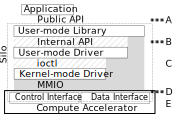
\includegraphics[width=.5\linewidth]{figures/silo.pdf}
	\caption{An accelerator silo. The public API and the interfaces with striped backgrounds are interposition candidates. All interfaces with backgrounds are proprietary and subject to change.}
	\label{fig:silo}
\end{figure}

Domain Specific Accelerator stacks are composed of layered components that
include a user-mode library to support an API framework and a driver to manage
the device. Vendors are incentivized to use proprietary interfaces and
protocols between layers to preserve forward compatibility, and to use
kernel-bypass communication techniques to eliminate OS overheads.

Scheduling and resource allocation on DSAs are typically not managed by the
CPU-based Operating System. Instead resource allocation is primarily under the
control of a combination of the proprietary CPU-based runtime (user-space and
kernel), and the controller on the DSA itself. DSAs typically contain an
entire software stack on the hardware module, which is hidden from the
programmer. This stack is used to implement a command-based programming
interface that enables the vendor's CPU-based control software for scheduling
and resource allocation.

End users work with the DSA almost entirely in higher level languages,
typically the language the DSL is embedded in (e.g., Python for Google's TPU,
C/C++ for Nvidia and AMD GPGPUs). The DSL/API is supported by a compiler
(which converts the user's program to the the ISA of the computation units on
the DSA), a user-space runtime and a kernel module (which work together to
implement the user-space API, and control the DSA).

\section{DSA Virtualization}

Despite mounting evidence of accelerator under-utilization~\cite{
underutilizingcloud, simultaneous_multikernel,improving_gpu,gpl,fiddle},
and abundant prior research into multiplexing Domain Specific Accelerators
(DSAs)~\cite{gpl,fiddle,zhang2018g, simultaneous_multikernel,improving_gpu,
yeh2017pagoda}, DSAs remain dedicated exclusively to a single guest in shared
computing environments. This section provides background on the well studied,
but mostly unresolved problem of GPGPU virtualization to explain this trend.

Existing GPU virtualization solutions~\cite{dowty2009gpu, VGML} support
graphics frameworks like Direct3D~\cite{directX}, OpenGL~\cite{openGLspec}.
In principle, there should be no fundamental difference between GPU
virtualization for graphics versus \emph{compute} workloads, as ``compute
shaders'' are implemented by the hardware as an additional stage in the
graphics pipeline~\cite{gpu_shader}.
In practice, they have significantly different goals:
for graphics, virtualization designs target an interactive frame rate (18-30
fps~\cite{frame_rate}); for GPGPU compute, virtualization designs must
preserve the raw speedup achieved by the hand-optimized GPGPU application,
which is a considerably harder target to hit. As a result, GPGPU virtualization
remains an open problem. While graphics devices have long enjoyed well-defined
OS abstractions and interfaces~\cite{winGDI}, research attention to OS
abstractions for GPGPUs~\cite{rossbach2011ptask, dandelion,
silberstein2013gpufs, timegraph, gdev, gpunet} has yielded little consensus.
Persistent vendor-specificity of programming frameworks further impedes both
interposition and compatibility.

\subsection{Inefficacy of Traditional GPGPU Virtualization Techniques}
An ideal GPGPU virtualization design would require no modification of
guest applications, libraries and OSes (compatibility), arbitrate fair and
isolated sharing of GPU resources between mutually distrustful VMs (sharing
and isolation) at the native performance of the hardware (performance), while
allowing virtualized software and physical hardware to evolve independently
(encapsulation).
We briefly describe each technique, and look at their strengths and
shortcomings in this section. Refer to Related Work (\S~\ref{sec:related}) for
details on individual prior work under each technique.

\subsubsection{Pass-through}
PCIe pass-through, the current \emph{de facto} standard technique for GPGPU
virtualization, provides a VM with full exclusive access to a physical GPU.
The GPU's hardware interface is directly exposed to the guest OS, and
therefore can't be multiplexed as the hypervisor does not interpose \emph{any}
interface. Virtualization hardware extensions (e.g., Intel VT-d~\cite{
abramson2006intel}) are device-agnostic, making PCIe pass-through easily
adaptable to any DSA. Pass-through provides native performance at the cost of
\emph{sharing, interposition, compatibility and isolation}.

\subsubsection{Device emulation}
Device Emulation~\cite{bellard2005qemu} provides a full-fidelity
software-backed virtual device which yields excellent compatibility,
interposition, and isolation. However, device emulation can't support hardware
acceleration making it untenable for virtualizing GPGPUs.

\subsubsection{Full virtualization}
The hypervisor interposes GPU's hardware interface to provides a virtual
environment in which unmodified GPGPU programs run on unmodified guest
software stacks.
For DSAs, this interface tends to be memory mapped I/O (MMIO), necessitating
trap-based interposition (e.g. using memory protection or de-privileging),
leading to devastating performance slowdowns (e.g., 100$\times$ slowdown with
GPUvm~\cite{suzuki2014gpuvm,yu2017fullvirt}). DSA hardware interfaces tend to
be proprietary and device-specific, so full virtualization based solutions
have poor compatibility, even across different devices of the same type (e.g.
AMD vs NVIDIA GPUs). Full virtualization solutions also typically rely on
reverse engineering of proprietary control interfaces, rendering them
extremely tedious to build, maintain and evolve.

\subsubsection{Mediated pass-through}
A hybridization of pass-through and full virtualization, Mediated
pass-through~\cite{gVirt,mdev-mvme,vpio} uses pass-through for data plane
operations, and provides a privileged control plane interface for sensitive
operations. Mediated pass-through can preserve some of the raw speedup of
acceleration and allows guests to use native drivers and libraries.
However, limited interposition limits a hypervisor's ability to effectively
manage resource sharing. More importantly, hardware support is required. To
our knowledge, Intel integrated GPUs are the only accelerators with such
support.

\subsubsection{Para-virtualization}
Rather than interposing an existing interface in the stack,
para-virtualization~\cite{suzuki2014gpuvm,dowty2009gpu,vasila-gvm16,
vmm-independent-gfx-vee07,harel-efficient13atc,exitless-paravirtual-io,
vmm-bypass-atc06, self-virt-hpdc07,vmware-hosted-io-atc01,
direct-access-virt-io-atc08, paradice} \emph{creates} an efficiently
interposable interface in software and adjusts adjacent stack layers to use
it. The driver and runtime libraries in every supported OS must be
modified to work in concert with the virtualization layer.
Para-virtualization enables encapsulation of diverse hardware behind a single
interposable interface, but compromises compatibility. Guest software must be
modified, and the para-virtual device interface must be maintained as
interfaces evolve.
For example, VMware's SVGA II~\cite{dowty2009gpu} encapsulates multiple GPU
programming frameworks, but keeping up with the evolution of those frameworks
has proved untenable: SVGA remains multiple versions  behind current
frameworks~\cite{vmware_version,svga_guest}.

\subsubsection{API Remoting}
User-space API Remoting based virtualization designs interpose
application-level APIs (e.g. CUDA, OpenCL) by shimming a dynamic library and
remote them to the corresponding framework in the host~\cite{shi2012vcuda,
gupta2009gvim, gVirtuS}, on a dedicated appliance VM~\cite{vmCUDA}, or on a
remote server~\cite{rCUDA,rCUDAnew,GridCuda,kim2012snucl,VCL,Duato2009,Li2011}.
API Remoting is similar to RPC~\cite{nfs,sunrpc} or system call
interposition~\cite{paradice, nooks, rio, vrio}.
Limited interposition frequency, batching opportunities~\cite{rCUDA} and
high-speed networks~\cite{deplyrcuda, bitfusion} reduce overheads, making this
class of designs appealing to industry. Dell XaaS~\cite{xaas}, BitFusion
FlexDirect~\cite{bitfusion}, and Google Cloud TPUs~\cite{cloud-tpu} currently
use it to support GPUs, FPGAs, and TPUs.
However, API remoting compromises compatibility if multiple APIs or API
versions must be supported. Moreover the technique bypasses the hypervisor,
giving up the interposition required for hypervisor-enforced resource
management. Our experiments with commercial systems like BitFusion
FlexDirect~\cite{bitfusion} show vulnerability to massive unfairness
pathologies. Figure~\ref{fig:bitfusion_unfairness} shows the problem on an
NVIDIA GTX 1080: FlexDirect is unfair (up to 88.1\%) when running two
applications with different kernel run-lengths (126.3~ms/kernel vs 0.18~ms/
kernel in the worst case).

\begin{figure}[!t]
	\centering
	\includegraphics[width=.8\linewidth]{figures/bf_unfairness.pdf}
	\caption{Unfairness in slowdown between \lstinline|needle| and \lstinline|hotspot| applications in separate VMs running GPU kernels iteratively
    with BitFusion FlexDirect.
    When running alone, \lstinline|hotspot| has throughput of 126.3~ms/kernel.
    Fairness is calculated by $\left|s_1-s_2\right| \mathbin{/} (s_1+s_2),$
    where $s_i$ is the slowdown of application $i$ when running concurrently.
    \aak{remove AVA from this figure.}}
	\label{fig:bitfusion_unfairness}
\end{figure}

Deferring enforcement to a trusted surrogate in the host or remote machine is
a tenable alternative. However, the co-ordination required to integrate with
hypervisor-level resource management means that current solutions do not
support it, and the engineering effort required would be substantial.
Existing accelerator API remoting systems are by themselves massive
undertakings without any hypervisor integration: systems like Bitfusion
FlexDirect~\cite{bitfusion}, and rCUDA~\cite{rCUDA} reflect multi-year
system-building efforts.

\subsubsection{Hardware virtualization support}
Hardware support for virtualization (e.g., Single Root I/O Virtualization (
SR-IOV)) enables a single physical device to present itself as multiple
virtual devices. A hypervisor can manage and distribute these virtual devices
to guests, effectively deferring virtualization, scheduling, and resource
management to the hardware. NVIDIA and AMD both ship GPU cards targeted at the
VDI market that use SR-IOV to export multiple virtual GPUs from the hardware.

SR-IOV exhibits close to native performance~\cite{XenSRIOV}, but this is
achieved at the cost of interposition --- the hypervisor can't interpose
on any interactions with the hardware. SR-IOV also suffers from the multiple
administrator problem: the hardware controller and the hypervisor/OS may make
mutually inconsistent decisions leading to unpredictable behavior.
SR-IOV provides an interface and protocol for managing VFs, but the device
vendor must \emph{implement} any cross-VF sharing support \emph{in silicon}.
The technique can provide strong virtualization guarantees~\cite{dong2012high,
dong2008sr}, but hardware-level resource management is inflexible and slow to
evolve: current implementations are trivially vulnerable to fragmentation and
unfairness pathologies that cannot be changed.

\begin{figure}[!t]
	\centering
  \vspace{-0.5em}
	\includegraphics[width=.75\linewidth]{figures/qat_unfairness.pdf}
    \vspace{-.2cm}
	\caption{Throughput achieved by three instances of QATzip (running in VMs with SR-IOV pass-through) with different block sizes, running separately (\textbf{\texttt{Uncontended}}) and concurrently (\textbf{\texttt{Contended}}). Slowdown during concurrent execution is dependent on block size, i.e., the QAT HW scheduler cannot guarantee fairness.}
	\label{fig:qat-unfairness}
\end{figure}

Hardware designers tend to favor simple resource management policy
implementations, easily leading to pathologies. To illustrate the problem, we
measured compression throughput when three VMs contend on an Intel
QuickAssist~\cite{qat} (with SR-IOV). The three VMs configured the accelerator
to compress at different chunk sizes. Figure~\ref{fig:qat-unfairness} shows
the results of this experiment, with and without contention. Each VM was
assigned a PCIe Virtual Function (VF) exposed by the same Physical Function
(PF), causing the hardware to schedule requests round-robin. When there is no
contention, each application achieves a similar throughput. However, when the
3 applications were executed concurrently, the throughput achieved was a
function of offload chunk size used, \emph{yielding unfairness that cannot be
fixed without changing the hardware}.

Further, evidence is scant that broad SR-IOV support will emerge for
accelerators: only two current GPUs support it~\cite{amdfirepro,nvidiagrid},
none of the TPUs we evaluate support it; and SR-IOV \emph{interface} IP blocks
from FPGA vendors (used by~\cite{vu2014enabling,zazo2015pcie,vfpgamanager,
huang2009fpgavirt}) do not implement resource management.

\section{Summary}

Interposing opaque, frequently-changing interfaces communicating with memory
mapped command rings is \emph{impractical} because it requires inefficient
techniques and yields solutions that sacrifice compatibility.
Accelerator stacks are effectively \emph{silos} (Figure~\ref{fig:silo}), whose
intermediate layers \emph{cannot be practically separated} to virtualize the
device. Most current hardware accelerators feature some hardware support for
virtualization: primarily for process-level address-space separation, and in a
small handful of cases, SR-IOV. A central premise of this dissertation is that
hardware support for process-level isolation \emph{could} suffice to support
hypervisor-level virtualization as well, but the silo-ed structure of current
accelerator stacks prevents it.
While hardware support for virtualization is the desired end game, we do not
expect a better standard for such support to emerge soon: incentives for
investing in the significant engineering effort required for such a standard
are scarce. This dissertation focuses on virtualization schemes that can be
purely implemented in software so as to sidestep this challenge.
%% !TeX root = ../dissertation.tex
\section{Motivation}
\label{sec:motivation}

\begin{figure}[!th]
	\centering
	\includegraphics[width=.9\columnwidth]{images/shared-training.png}
	\caption{{\footnotesize Three TensorFlow workloads sharing an NVIDIA Tesla GPU. \aak{Apologies for being brutal, but this is pretty weak sauce. The data is noisy/inconclusive at best. I understand the reason to have this graph, but unless we can draw out some patterns (e.g. combinations that under-utilize the K20c should have much worse under-utilization on the p100 --- that shows that the problem is getting worse.) from the graph, it's hard to see any signal here.}}}
	\label{fig:motivation}
\end{figure}

\textbf{Fallacy:} \emph{most GPU workloads can fully utilize a GPU.}
This is a common misconception that is often touted to justify
the use of techniques that \emph{expose} dedicated GPU hardware~\cite{AWS-gpu}
rather than \emph{virtualize} them.
% to enable sharing it across protection domains.
On the contrary, the compute density of GPUs continues to grow at a pace
that suggests that it is almost certain that under-utilization of GPU
resources will be a major pain-point for cloud providers in the future, if it
already isn't.

To illustrate the opportunity, we co-scheduled three TensorFlow~\cite{
abadi2016tensorflow} programs --- MobileNet, ResNet50, InceptionV3 --- in
pairs, on a single NVIDIA Tesla~\cjr{TODO get machine
details} GPU~\footnote{Execution times for all the programs are on the order of hundreds of seconds. The batch size was 32. The \texttt{allow\_growth}
option was enabled to prevent TensorFlow from pre-allocating all GPU
memory and \texttt{gpu\_memory\_fraction} was set to 0.5 in GPUOptions to
ensure at most half of the GPU memory is used for each co-scheduled program.}, and measured the execution (inference) time.
% , all from TensorFlow's \texttt{tf.keras.applicat\-ions},

Figure~\ref{fig:motivation} shows the relative execution time of all possible
co-schedules of these workloads. Considering their total serial execution time
on dedicated hardware to be 2$\times$, cases where relative times exceed
2$\times$ indicate slowdown due to contention; those that are under 2$\times$
indicate under-utilization. Under-utilization of GPU resources indicates a
failure to fully leverage the hardware (e.g. by co-scheduling GPU kernels with
complementary resource demands). While slowdown from contention does occur (at
most 10\% of total serial execution time), \( \frac{4}{9} \) of the cases
yield \emph{speedup}. The data are evidence that the cost of sharing is
tolerable and under-utilization is real. Our findings are corroborated by
others~\cite{long-list-of-citations-hangchen-dug-up}. We note that newer GPU
hardware, such as NVIDIA Volta V100~\cite{volta-nvidiaweb}, have many times
the compute density of the GPUs we tested, and the growth trend is projected
to continue.
% !TeX root = ../dissertation.tex
\section{Design}
\label{sec_design}
\label{sec:trillium_design}

\Trillium exports an abstract virtual device and a para-virtual guest driver,
which we use to interpose and forward the OpenCL and CUDA APIs to the host.
Unlike SVGA, which requires translation
layers to ensure that all graphics frameworks APIs can be mapped to the SVGA protocol,
Trillium forwards the lowest layer in the GNU/Linux Graphics stack: the pipe-driver,
effectively remoting OpenCL/CUDA API calls in the guest to the OpenCL/CUDA library in the host.

%\Trillium is composed of a virtual GPU device, and a para-virtual guest driver
%which we use to interpose and forward a GPGPU API through the virtual
%device implementation to the host. Unlike SVGA, which requires translation
%layers to map graphics APIs to the SVGA protocol, Trillium forwards
%Mesa3D pipe-driver functions directly, effectively remoting an OpenCL API
%implementation in the Mesa stack to an OpenCL implementation in the host.

%% \item The historical approach of translating/tunneling other graphics APIs
%% 	over the SVGA protocol is unnecessary, and the protocol can simply be
%% 	extended directly with GPGPU APIs without compromising
%% 	other important properties of the design.

% \Trillium is heavily influenced by the SVGA design, but
Our experience implementing the required TGSI vISA support in the Mesa
graphics stack led us to believe that the TGSI layer is unnecessary.
Not only does this translation introduce additional complexity in the guest
stack, it also hurts performance, as we demonstrate in Section~\ref{sec:eval}.
The guest OpenCL compiler cannot target the native GPU architecture,
and semantic information is lost to the host compiler.
% Because SVGA's native ISA is TGSI, supporting GPGPU workloads in SVGA requires
% GPU code to be expressed in TGSI, rather than in the ISAs produced
% by vendor-specific runtimes (e.g. CUDA's \texttt{PTX} and
% \texttt{SASS}, or AMD's \texttt{SPIR}).
Further, while incorporating a TGSI compiler is possible in open frameworks like OpenCL,
the task is significantly more daunting for closed frameworks like CUDA.
Attempts to translate between TGSI and NVIDIA SASS in the reverse-engineered Nouveau driver
understandably results in code that is significantly less performant
than that produced by the proprietary stack.

\Trillium takes a different approach:
% rather than build a compiler for guest to a virtual ISA which must then be translated in the hypervisor,
% of the production compiler for the actual physical device and
\Trillium forwards API calls for compiling OpenCL code to the hypervisor.
The OpenCL compiler in the host OpenCL framework
(optimized for the physical hardware by the hardware vendor)
is invoked on the forwarded OpenCL code to lower it directly to the physical device ISA.
% If the host OpenCL driver does not support a compiler, \Trillium uses LLVM IR as the virtual ISA.

%\begin{figure}[!th]
%	\centering
%	\includegraphics[width=.8\linewidth,trim={0 0 0 0},clip]{images/design/trillium_design.pdf}
%	\caption{{\footnotesize The design of \Trillium.
%            \cjr{FIXME: get designs in position as discussed with Hangchen. }}}
%	\label{fig_trillium} \end{figure}

Figure~\ref{fig_trillium} shows the Trillium design layers in a
generic hypervisor stack. The OpenCL API is forwarded from the
driver similar to the SVGA model.  The OpenCL compute kernel (to be
run on the GPU), can be passed through to the host via hypercalls in
the driver, without being translated to any vISA, where it will
be translated and optimized for the physical GPU in a virtual appliance (Dom~2 in Figure~\ref{fig_trillium}).

\Trillium does not currently guarantee performance isolation and relies on the hardware scheduler.
% task is handed to the hardware.
Performance isolation can easily be implemented via a rate-limiting API scheduler in the
hypervisor, such as in GPUvm~\cite{GPUvm}.

%% \aak{Chris, what level of detail do you want to go to? I'm keeping it minimal
%% here so as to not risk de-anonymizing you. Mentioning that you built this model
%% at VMware will bring questions of why we didn't measure that system instead.}

% \begin{figure}[!th]
% 	\centering
% 	\includegraphics[width=\linewidth,trim={9cm 4cm 9cm 4.5cm},clip]{images/trillium/trillium_classic_single_node.pdf}
% 	\caption{{\footnotesize The design of Trillium Classic.}}
% 	\label{fig_trillium_classic2} \end{figure}


% \subsection{Impact of GPU virtual ISAs}


% % \begin{table}[!th]
% % 	\centering
% % 	\begin{tabular}{l|l|l|l|l|}
% % 		\cline{2-5}
% % 		& Init & MemCpy & Kernel & Total \\ \hline
% % 		\multicolumn{1}{|l|}{ocl+mesa} & \multicolumn{1}{r|}{5.4x} & \multicolumn{1}{r|}{6x} & \multicolumn{1}{r|}{14.5x} & \multicolumn{1}{r|}{7x} \\ \hline
% % 	\end{tabular}
% % 	\caption{Slowdown of Clover OpenCL runtime.}
% % 	\label{tb_clover_slowdown}
% % \end{table}

% The design trades off compatibility: the goal of the virtual TGSI ISA
% for the virtual GPU is to function as universal IR, so that a guest
% compiler is able to produce code that can always be finalized below
% the virtualization layer to a native ISA for the physical GPU. While
% conceptually attractive, the design decision is only effective if
% components elsewhere in the stack (GPU runtimes, compilers, drivers,
% etc.) actually standardize on it.  At present, NVIDIA and AMD GPGPU
% stacks both suppport virtual and native ISAs, but \emph{different}
% ones, neither of which is TGSI, making TGSI effectively an additional
% layer of virtualization on the ISA. We also observe that because both
% AMD and NVIDIA compilers are built on LLVM, there is an opportunity
% for standardizing on LLVM IR as the common IR, which would naturally
% recover the compatibility ceded by the \Trillium design.

% -*- fill-column: 85; -*-
%!TEX root = ../dissertation.tex

\graphicspath{{images/}}

\subsection{Communication Transport}
\label{s:design_transport}

\AvA relies on an abstract communication channel that defines how
calls, and their associated data buffers, and results are sent, validated, and received.
%The channel interface provides primitives to send/receive commands.
% to marshal/unmarshal function arguments and  AMP: Our channel does not provide marshalling other than buffer attachment, so I don't think it's important and could confuse people as marshalling can imply things like encoding strings or numbers.
The channel provides an interposition point to track resources and invoke policies from the \Lapis specification.
Using an abstract interface allows hypervisor developers to choose the best available communication transport
(e.g., shared memory FIFOs vs RDMA).
While the channel explicitly requires that all communication between the guest
and the \worker must take place through the router, no assumptions are made
about the actual location of components, which may be
disaggregated.


% \subsection{Callbacks}
%\label{s:callback}
\AvA communication is bidirectional: it must support function callbacks from the \worker to the guest library, because
callbacks are fundamental in many frameworks, e.g., TensorFlow,
and must be run in the guest VM. % (instead of the \worker) to
%protect host domain from malicious code.\cjr{I think it would also be incorrect to run them anywhere else.}
In \AvA, the transport handles two types of payloads: \emph{commands} which contain opaque arguments and metadata for calls (e.g., thread ID and function ID) and \emph{data} which contains buffers referenced from the arguments (e.g., bulk data).

\subsection{Sharing and Protection}
\label{s:protection}

\AvA re-purposes process-level isolation mechanisms (e.g. memory protection)
provided by the accelerator silo when it is available to simplify supporting cross-guest
isolation. We anticipate that emerging accelerators will support process-level isolation, as all GPUs do today.
% We reiterate that lack of hardware virtualization support is not the obstacle for accelerator virtualization,
% but stack structure is: if and when all accelerators support process-level virtualization in hardware,
% \AvA will still be necessary because vendor stacks do not expose the interfaces required to take advantage
% of that support.
%~\cjr{This last sentence is important, but too long.}
%~\cjr{But, we're going to keep it.}
For accelerators that do not natively support process-level isolation,
\AvA can still share device, relying on semantic information from additional \Lapis descriptors
to generate code that supports coarse-grain time-sharing, leveraging the same state capture techniques we use for VM migration (\S\ref{s:migration}).
% A descriptor on functions that create and destroy connections to hardware allows
% the \CAvA to insert additional logic in the device open/close calls to
% transparently spin until the device becomes available.
This solution admits no concurrency between tenants, but enables protected
sharing for devices which cannot otherwise be shared.

\subsection{Scheduling and Resource Allocation}
\label{s:rate_limit}
\label{s:api_throttling}

\AvA can enforce policies (e.g., rate limiting) on shared resources,
e.g., device execution time, by tracking resource consumption and invoking
policy callbacks that change how API calls from
guests (\S\ref{sub:scheduling}) are scheduled.
The developer provides policy callbacks in the \Lapis specification, and uses descriptors to identify how resources are consumed.
% ~\cjr{I assume this is a callback or something? The spec can't provide an approximation, but it can provide a way to get it, right?} of
%of the shared resource.
When such a descriptor is unavailable, \AvA falls back to coarse-grained
estimation of resource utilization, for example, using wall-clock time to approximate device execution time.
%We expect even such a rough approximation to be sufficient for useful policy enforcement.
% \hyu{We should say we can do better than wall-clock approximation.}
% \AvA uses adaptive call rate limiting, based on proportional time-sharing
% and feedback control~\cite{scheduling_survey} (see \S~\ref{sub:scheduling}).

% The \AvA router schedules only API function calls, like previous API
% remoting systems. However, unlike previous systems, the router runs in the
% hypervisor, and can be integrated/federated with schedulers for other resources to
% improve locality and performance.

\subsection{Memory Management}

To support memory sharing on devices with onboard memory, \Lapis resource usage descriptors
enable generated code to track the device memory
allocated to each guest VM. %based on the resource usage description in \Lapis. In this scenario, the router would rely on the
%\worker to notify it of all allocation and deallocation of device memory.
Resource accounting code is auto-generated from semantic knowledge of
the device memory allocation APIs (such as, memory types and how to compute size
of buffer) provided by descriptors in the API specification.
%If a device memory allocation request would exceed the guest's quota,
%the \worker returns the appropriate Out-of-Memory (OOM) error for the allocation.

%\beginchanged
% -*- fill-column: 85; -*-
%!TEX root = ../dissertation.tex

\begingroup % A group to prevent \txt from leaking into following files.
\newcommand{\txt}[1]{\textrm{\it #1}}
\newcommand{\halfvspace}{} % \vspace*{0.25em}
\newcommand{\halfhspace}{\hspace*{0.25em}}
\newcommand{\spec}{\lstinline[language=C,style=nwspecc,columns=fullflexible]}

\graphicspath{{images/}}

\section{\CAvA and \Lapis}
\label{s:api}
\label{s:compiler}

The \AvA toolchain
comprises a language (\Lapis), a compiler (\CAvA), and a runtime library.
% AMP: The runtime is not written in Lapis. (It will be in Lapis 2, which I may well have mentioned at some point)
\CAvA accepts code written in \Lapis (\textbf{L}ow-level \textbf{API} \textbf{S}pecification), and generates C
source for an API-specific remoting stack that implements the \hira design.
\Lapis extends C declarations with descriptors to express a broad range of semantic information
necessary to generate that stack.
This includes information captured by traditional IDLs (e.g., function parameter semantics and data layout),
as well as information required for accelerator virtualization that is not expressible in existing IDLs.
% \Lapis is not inherently specialized for accelerator API remoting--the additional semantics
% required for \AvA are expressed in terms of more general language-level primitives:
% however, to simplify discourse, we will focus only on features relevant to \AvA.

To understand how \AvA relates to other IDL-based API-remoting techniques,
it is useful to compare it to the Sun Network File System~\cite{Sandberg:1988}.
NFS supports remote access to the the file system using
an IDL to specify API semantics and a compiler to automate code generation. NFS and \AvA share a number of
key challenges. Both must marshal and transfer function calls and arguments, handle asynchrony,
refactor functionality and (potentially implicit) state across newly decoupled components. Both must
preserve the resource management and sharing support expected for a resource managed by system software.

However, key differences between \AvA and NFS arise around additional virtualization requirements and
limitations in the design space.
For example, virtualization requires that \AvA be able to capture of
sufficient API-level state to enable features like live VM migration.
Key techniques used by NFS to deal with implicit state and
resource management are impractical \AvA.
NFS mostly \emph{eliminates} implicit state by altering the API,
e.g. replacing functions using implicit seek pointers with stateless read/write functions and offset parameters.
To deal with resource management, sharing, and compatibility challenges,
NFS \emph{introduced} the VFS layer, providing
an application-transparent interposition point at which to centralize or delegate that functionality using code written
to run at that layer. \AvA cannot alter APIs, so it exposes language-level features for dealing with implicit state.
\AvA cannot introduce new abstraction layers due to vendor opacity and API diversity: so the
resource management and sharing policy are expressed at the language layer as well.

% \paragraphbe{OS interposition.} A significant challenge faced by NFS was lack of a well-defined
% OS-level API for the file system, which is necessary for preserving OS-level resource management of the file
% system and providing compatibility at a software layer that minimizes application level change. While \AvA
% has the same problem (there are no standard OS-level interfaces for accelerators), the NFS designers had
% the luxury of simply defining one: the VFS layer is introduced for precisely this purpose.

% \paragraphbe{Difficult-to-capture API semantics.} API prototypes in a native header file do not fully
% specify the semantics of that API for a number of reasons. Some of missing semantics are
% straightforward to provide with an IDL specification, e.g. \texttt{in/out} semantics for arguments are absent,
% type layout for serialization, and relationships among individual function arguments such as buffer pointers and sizes.
% Some missing semantics are more difficult to capture in an IDL, for example API functions may
% refer to or manipulate context that is carried across API calls, such as seek pointers for \texttt{read} and \texttt{write} calls,
% which presents a design challenge for how to factor such implicit state\amp{context?} across the client/server boundary.
% Unlike NFS, which had the luxury of simply changing APIs to minimize implicit state (e.g. by replacing seek position with
% explicit offset parameters, or piggy-backing generation numbers on client file handles), \AvA does not have the
% luxury of changing APIs. Moreover, \AvA must contend with a number of additional requirements not
% present in NFS: enabling \emph{hypervisor-level resource management} requires semantic knowledge the relationship between
% API calls and accelerator-level resource management (e.g. how much memory is allocated, what fraction of the compute
% cycles are dedicated to individual guests), semantic knowledge of API-level \emph{object lifetimes} to support
% features such as live migration, and the ability to express resource management \emph{policies} that can be enforced by the hypervisor.

% While extending an existing IDL would provide \AvA with necessary semantics to deal with
% basic parameter marshalling, we know of none that capture all the semantics required to enable
% state tracking for device-side objects, abilitiy to express complex implicit API state, and
% support for expressing and enforcing resource management polcies. Moreover, while the guest library
% and API servers generated by \CAvA are analogous to the stubs and skeletons created by an
% IDL compiler, \AvA requires a backend specialize to additionally generate device driver code, and
% policy hooks to run in the hypervisor. Consequently, we chose to design a new language and compiler that
% meets these needs.

% \cjr{Present CAvA and LAPIS as a development platform: runtime library support is a key element.}

% -*- fill-column: 85; -*-
%!TEX root = ../main.tex

\begin{figure}
%@@cuMemcpyHtoDAsync(CUdeviceptr dst, void *src,|\label{line:cuMemcpyHtoDAsync}|
%           size_t size, CUstream stream)@@ { 
%  async; success(CUDA_SUCCESS);
%  argument(src) { in;|\label{line:src-in}| buffer(size); lifetime_manual; }
%  register_buf(async_HtoD, stream, src, size); }
\begin{lstlisting}[language=C,style=nwspecc,columns=flexible,belowskip=-0.5em,aboveskip=-0.5em,mathescape,basicstyle={\scriptsize\ttfamily}]
continuous_rc device_memory;
instantaneous_rc kernel_invocations;|\label{line:declare_rc}|
policy("policy_kern.c");|\label{line:scheduler_code}|
struct fn_arg_info {
  // CUfunction type information, filled by other LAPIS code
  int fn_argc;
  char fn_arg_is_handle[64];
  size_t fn_arg_size[64];
};
declare_metadata(struct fn_arg_info);
buf_registry async_DtoH;
type(CUdeviceptr) { handle; }|\label{line:cudeviceptr-handle}|
@@cuMemAlloc(CUdeviceptr *pp, size_t size)@@ { 
  allocates_rc(device_memory, size);|\label{line:allocates_rc}|
  argument(pp) { out; element { obj_record; allocate; } } }
@@cuMemcpyDtoHAsync(void* dst, CUdeviceptr src,|\label{line:cuMemcpyDtoHAsync}| 
                    size_t size, CUstream stream)@@ {
  async; success(CUDA_SUCCESS);|\label{line:success}|
  argument(dst) { no_copy;|\label{line:dst-nocopy}| buffer(size); lifetime_manual; }
  register_buf(async_DtoH, stream, dst, size); }
@@cuLaunchKernel(CUfunction f,
    uint gridDimX, uint gridDimY, uint gridDimZ,
    uint blockDimX, uint blockDimY, uint blockDimZ,
    uint sharedMemBytes, CUstream hStream,
    void **kernelParams, void **extra)@@ {
  async; consumes_rc(kernel_invocation, 1);|\label{line:consume_rc}|
  argument(kernelParams) {
    in; buffer(metadata(f)->fn_argc);
    element {
      if (metadata(f)->fn_arg_is_handle[index]) {
        type_cast(CUdeviceptr*); buffer(1);
      } else {
        type_cast(void*); buffer(metadata(f)->fn_arg_size[index]);
      } } }
  argument(extra) { in; ... } }
@@cuStreamSynchronize(CUstream stream)@@ {
  contextual_argument void** bufs =|\label{line:sync-bufs-1}| get_bufs(async_DtoH, stream);|\label{line:sync-bufs-2}|
  argument(bufs) {
    in; buffer(get_n_bufs(async_DtoH, stream));
    element { 
      buffer(get_buf_size(async_DtoH, stream, index));
      out; deallocate; } } }|\label{line:dst-buf-out}|
\end{lstlisting}
% no_copy; buffer(get_async_free_buf_size(stream, index));
\caption{
An example \speclang description for the CUDA driver API.
Code elements in {\lapiskeywordstyle bold blue} are \speclang keywords, elements in {\lapisstdlibstyle italic green} are runtime library calls, 
elements in {\lapisprototypestyle gray} are function prototypes incorporated by \compiler from the original CUDA header file,
and the remaining code is programmer-provided \speclang.
The variable \spec|index| is a \speclang builtin which provides the index of the current element of a buffer.
The specification of the argument \spec|extra| to \spec|cuLaunchKernel| is complex due to alignment and padding, and is elided from this example for clarity. 
%The specification of \spec|extra| is overall very similar to the specification of \spec|kernelParams|.
The file \spec|policy_kern.c| is shown in Figure~\ref{fig:scheduler_example}.
}
\label{fig:lapis-values-example}
\label{fig:spec_example}
\vspace*{-0.5em}
\end{figure}


\subsection{\Lapis}

A developer writing a \Lapis specification must be concerned with
capturing and expressing API semantics that fall roughly into four categories:
argument and data marshalling, asynchrony, explicit and implicit state,
and resource management policy.
To illustrate how \CAvA, \Lapis, and the runtime library,
work together to address these concerns, we will use a running example that
uses the CUDA driver API in an idiomatic scenario. The example allocates GPU memory (\texttt{cuMemAlloc}), makes
asynchronous calls using CUDA streams to transfer data before (\texttt{cuMemcpyHtoDAsync}) and after (\texttt{cuMemcpyDtoHAsync}) launching a kernel (\texttt{cuLaunch\-Kernel}),
and synchronizes the stream (\texttt{cuSynchronize\-Stream}).
The \Lapis source for the four of the five CUDA API functions required is shown in \autoref{fig:lapis-values-example}. We
elide source for \texttt{cuMemcpyHtoDAsync} because it is conceptually similar to \texttt{cuMemcpyDtoHAsync}.

\Lapis extends C types and function prototypes with information to serialize arguments and return values,
and manage user-defined metadata on API-level objects such as GPU kernels or memory buffers. The latter can be used to
specify the higher-level semantics and behaviors required for virtualization such as how to capture, transfer, and synchronize implicit state.
Descriptors are embedded in \Lapis function declarations,
can be flexibly scoped (\autoref{tab:lapis-scope}), and
applied to values (\autoref{tab:lapis-values}) or functions (\autoref{tab:lapis-functions}).
%A descriptor can also use a \Lapis keyword to apply to an \spec|argument|, an \spec|element| of a buffer, or all instances of a \spec|type|.
Descriptors can be conditional using an \spec|if| statement.
In the following discussion of \Lapis descriptors, we use the term ``this function'' to refer the function
being described or the function whose argument is being described.

\paragraphbe{Marshalling and Managing Values and Objects.}
\Lapis value descriptor usage is illustrated by the CUDA function \spec|cuMemcpyDtoHAsync| defined in \autoref{fig:lapis-values-example} (Line~\ref{line:cuMemcpyDtoHAsync}).
The argument \spec|src| is only used by the application through API calls
(\AvA does not currently support UVM, see \S\ref{s:limitations} for details).
This is true of the type \spec|CUdeviceptr| in general, so it
is expressed on line~\ref{line:cudeviceptr-handle} with \spec|type(CUdeviceptr) { handle; }|.
The \spec|handle| descriptor enables \AvA to generate code that implements an indirection layer for accessing it.
The argument \spec|dst| is a pointer to an application buffer of length \spec|size|; this is expressed on line~\ref{line:dst-nocopy} with \spec|argument(dst) { no_copy;| \spec|buffer(size); }| which selects the argument \spec|src| and specifies it as a \spec|buffer| of \spec|size| length.
The buffer will be copied back to the application later so it is \spec|no_copy| here.
Because the function is asynchronous (see below), the buffer for \spec|src| in the \worker must exist at least until the copy has completed:
the descriptor \spec|lifetime_manual| on line~\ref{line:dst-nocopy} states that the specification will indicate when the buffer is no longer needed using \spec|deallocate| (line~\ref{line:dst-buf-out}).
%On line \ref{line:src-in} \spec|in| informs \CAvA that the buffer will only be read by the call and should be copied from the application to the \worker before the call.
%The argument \spec|size| is a primitive value so \CAvA can simply copy its value directly from the application to the \worker. This is the default, so no descriptor is needed.
%The \spec|cuMemcpyDtoH| specification is similar except the types of \spec|src| and \spec|dst| are switched and the buffer argument is now annotated with \spec|out| since it will be written by the call and needs to be copied back to the application thereafter.

% -*- fill-column: 85; -*-
%!TEX root = ../main.tex

% NOTE: TexLive 2017 fails when a lstlisting environment is inside a table. This is fixed in 2018, but
% multirow still has the issue. Because of this, I'm using saveboxes for a bunch of listings just in case.
\newsavebox{\boxargumentsyntax}
\begin{lrbox}{\boxargumentsyntax}
\begin{lstlisting}[language=C,style=nwspecc,columns=fullflexible,numbers=none]
argument(x) {
  descriptors }
\end{lstlisting}
\end{lrbox}

\newsavebox{\boxelementsyntax}
\begin{lrbox}{\boxelementsyntax}
\begin{lstlisting}[language=C,style=nwspecc,columns=fullflexible,numbers=none]
element {
  descriptors }
\end{lstlisting}
\end{lrbox}

\newsavebox{\boxtypesyntax}
\begin{lrbox}{\boxtypesyntax}
\begin{lstlisting}[language=C,style=nwspecc,columns=fullflexible,numbers=none]
type(ty) {
  descriptors }
\end{lstlisting}
\end{lrbox}

\newsavebox{\boxifsyntax}
\begin{lrbox}{\boxifsyntax}
\begin{lstlisting}[language=C,style=nwspecc,columns=fullflexible,numbers=none]
if (pred) { 
  descriptors1
} else {
  descriptors2 }
\end{lstlisting}
\end{lrbox}

\begin{table}
  \centering
\resizebox{\columnwidth}{!}{
  \begin{tabular}{@{}p{1in} p{3in}@{}}
  \toprule
  Scope & \spec|descriptors| in this scope apply to ...  \\
  \midrule 
  \raisebox{-0.5em}{\usebox{\boxargumentsyntax}}  & the argument \spec|x|, called the described argument. \\
  \raisebox{-0.5em}{\usebox{\boxelementsyntax}} & the referenced value, called the described value; e.g., if applied to an argument \spec|x|, the descriptors inside apply to \spec|*x|. \\
  \raisebox{-0.5em}{\usebox{\boxtypesyntax}} & all values of type \spec|ty|. \\
  \raisebox{-1.7em}{\usebox{\boxifsyntax}} & \spec|descriptors1| apply only if \spec|pred| is true; \spec|descriptors2| apply otherwise. \\
  \bottomrule
  \end{tabular}
  }
  \caption{\speclang syntax which values descriptors apply to and when those descriptors apply.
  %\cjr{maybe we can refactor this   whole thing into the sentence that says descriptors are flexibly scoped.}
  }
  \label{tab:lapis-scope}
%  \vspace*{-1em}
\end{table}

% -*- fill-column: 85; -*-
%!TEX root = ../main.tex

\begin{table}
  \centering
\resizebox{\columnwidth}{!}{
  \begin{tabular}{@{}p{1in} p{3in}@{}}
  \toprule
  Type & The value is ... \\
  \midrule
  \spec|type_cast(ty)| & type \spec|ty| and should be cast in the generated code. \\
  \spec|handle| & an API object handle. \\
  \spec|buffer(size)| & a buffer of \spec|size| elements. \\
%  \spec|zerocopy| & an \AvA zero-copy buffer allocated using \spec|zerocopy_alloc|. \\
  \spec|in| & an input and should be copied from the application to the \worker before the call. \\
  \spec|out| & an output and should be copied from the \worker to the application after the call. \\
  \spec|no_copy| & a buffer which should not be copied. Useful when combined with lifetimes. \\
  \spec|lifetime_call| & a buffer which need only exist in the \worker for the length of the call. (default) \\
  \spec|lifetime_manual| & a buffer which should exist in the \worker until it is explicitly deallocated. \\
  \spec|allocate| & a buffer which calls to this function allocate. \\
  \spec|deallocate| & a buffer which calls to this function deallocate. \\
  \spec|zerocopy| & a buffer which should be in zero-copy memory. \\
  \midrule
  \end{tabular}
  }
\resizebox{\columnwidth}{!}{
  \begin{tabular}{@{}p{1in} p{3in}@{}}
  \multicolumn{2}{@{}l}{API Object Recording}\\
  \midrule
  \spec|obj_record| & This call should be recorded and associated with the described value. The recorded calls capture the implicit state of the value. \\
  \spec|obj_depends_on(obj)| & Add a dependency between the described value and \lstinline|obj|, enabling \lstinline|obj| to be recreated if the described value is needed. \\
%  \amp{This really is it. This has no sync implications, since playback is sequential. This is actually almost always inferred, we could actually leave it out of the paper pretty safely.}
  \spec|obj_state_cbs(write, read)| & Attach state serialization and deserialization (\spec|write| and \spec|read|, resp.) functions to the described value. The serialized data captures the explicit state of the value and may be used in combination with implicit state. \\
  \bottomrule
  \end{tabular}
  }
  \caption{\Lapis descriptors for specifying values and objects.}
  \label{tab:lapis-values}
%  \vspace*{-1em}
\end{table}


\paragraphbe{Asynchrony and Implicit State.} \Lapis supports descriptors
for expressing semantics that arise due to asynchrony.
Most commonly, these are expressed by applying descriptors to functions.
For example, \spec|cuMemcpyDtoHAsync| in \autoref{fig:lapis-values-example}
is asynchronous and can return \spec|CUDA_SUCCESS| before the copy completes;
this is expressed using \spec|async| and \spec|success| on line~\ref{line:success}.
%The function descriptors in \autoref{tab:lapis-functions} specify function-level metadata,
%such as kernel parameter types or other special processing needed to make a remote call.
%The \spec|sync| and \spec|async| descriptors specify if a call from the application can return immediately while \AvA handles the call asynchronously, e.g. to improve performance.
% by overlapping \worker and application-level work.
%Asynchronous functions return a value to the application as specified by the \spec|success| descriptor (line~\ref{line:success}).
%Forwarded API calls may need to copy buffers which are not explicitly exposed as arguments to the API function.
%For example,
%because the \worker maintains shadow copies of buffers,
Asynchrony can also create implicit API-level state whose semantics must be expressed.
\spec|cuStreamSynchronize| must copy buffers back to the guest if there are outstanding asynchronous copies.
Those buffers may not be updated in the \worker until the call completes, so copy-back must be delayed to this point.
This requirement is expressed by passing dependent buffers using \spec|contextual_argument| along with the normal explicit arguments. The \Lapis code on line \ref{line:sync-bufs-1}--\ref{line:dst-buf-out}
uses this technique along with runtime library functions to track buffers dependent on ongoing asynchronous copies.
\AvA supports zero-copy transport of buffers: if a buffer allocation is described with \spec|zerocopy|, \CAvA allocates zero-copy memory for the application-side buffer.
%this is an important optimization for high-throughput APIs (e.g., kernel bypass APIs).
%The current implementation only supports this in a few specific cases, but this is not a fundamental restriction.

%\autoref{tab:lapis-functions} also includes descriptors for resource accounting and sharing policy.
%These are used in \autoref{fig:lapis-values-example}.
\paragraphbe{Resource Management and Policy.}
\Lapis supports descriptors to express the resources consumed by API functions.
Resources may be either \emph{instantaneous} or \emph{continuous}.
Instantaneous resources are consumed by an API function implementation only once,
e.g., by executing a GPU kernel upon request. Accounting works by measuring resources used at each function invocation.
In general, instantaneous resources are used to control throughput in some way; e.g.,
limiting the amount of compute resource a client is allowed to use in a fixed interval of time.
Continuous resources capture the ability an API implementation to assign a resource to a client for a
period of time. Accounting for continuous resources tracks resources assigned to each client/VM.
For example, GPU memory is a continuous resource limited by available physical memory,
which needs to be allocated
according to a sharing policy that manages cross-VM contention for it.

\autoref{fig:lapis-values-example} uses descriptors to track kernel calls (\spec|cuLaunch|\-\spec|Kernel|) and GPU memory allocation.
In \Lapis, this is expressed using two resources and descriptors on functions to specify how much of each resource is consumed.
Line~\ref{line:declare_rc} declares a resource representing function invocation rate.
Line~\ref{line:scheduler_code} specifies the custom policy used to schedule function invocations.
Line~\ref{line:consume_rc} specifies that a call to \spec|cuLaunchKernel| counts as one unit of the \spec|kernel_calls| instantaneous resource.
Line~\ref{line:allocates_rc} specifies that a call to \spec|cuMemAlloc| allocates \spec|size| bytes of the continuous resource \spec|gpu_mem|.


%For some instantaneous resources (e.g., data transfer over the bus), the amount can be estimated based on the arguments to a function call (buffer size).
%For other instantaneous resources (e.g., computation), the amount needs to be computed after the fact by measure how long the call or calls took to complete.
%Because of this, resource usage descriptors may be handled after a call completes by some Lapis compilers.

To specify policies, developers provide functions that schedule API calls from different VMs based on the recorded resource usage of those VMs. In our current implementation, policy functions are specified as eBPF programs stored in a separate file and referenced from the \Lapis source using \spec@policy("policy_kern.c")@ at the top level. In future work, we plan
to extend \Lapis to express these policies directly. We currently use eBPF because it enables unprivileged code to run
safely in the hypervisor and is available today, enabling \AvA to be used without modifying the hypervisor and without trusting the developer. However, in principle, the same properties can be achieved using \Lapis
and will provide a significant complexity reduction for the developer.
%However, the policy function could be run in privileged context if it were trusted, or could be run using any other technique for unprivileged execution inside the kernel.
%However, eBPF is already available, avoiding the requirement of additional changes to the kernel.

% -*- fill-column: 85; -*-
%!TEX root = ../main.tex

% NOTE: TexLive 2017 fails when a lstlisting environment is inside a table. This is fixed in 2018, but
% multirow still has the issue. Because of this, I'm using saveboxes for a bunch of listings just in case.
\newsavebox{\boxutilitysyntax}
\begin{lrbox}{\boxutilitysyntax}
\begin{lstlisting}[language=C,style=nwspecc,columns=fullflexible,numbers=none,belowskip=-2.2em,aboveskip=-1em,mathescape]
utility $\txt{C declaration}$;
\end{lstlisting}
\end{lrbox}

\begin{table}
  \centering
\resizebox{\columnwidth}{!}{
  \begin{tabular}{@{}p{1.31in}@{}p{2.7in}@{}}
  \toprule
  Function & The function ... \\
  \midrule
  \spec|sync| & is synchronous: application calls wait for completion in the \worker. \\
  \spec|async| & can be asynchronous: calls will return immediately after call dispatch. \\
  \spec|success(v)| & should return \spec|v| when called with \spec|async|. \\
  \spec|contextual_argument| & has additional context that should be transported along with the normal arguments. This is used to copy values or buffers which are not explicitly arguments to the call, e.g., \spec|errno|.
%  Contextual arguments can be annotated as usual.
  \\
  \spec|allocates_rc(r, x)| & allocates \spec|x| units of the continuous resource \spec|r|. \\
  \spec|deallocates_rc(r, x)| & deallocates \spec|x| units of the continuous resource \spec|r|. \\
  \spec|consumes_rc(r, x)| & consumes \spec|x| units of the instantaneous resource \spec|r| during the call. \\
  \midrule
  Declarations & The statement declares ... \\
  \midrule
  \spec|continuous_rc r;| & a continuous resource \spec|r|. \\
  \spec|instantaneous_rc r;| & an instantaneous resource \spec|r|. \\
  \usebox{\boxutilitysyntax} & a global utility function or variable that is not part of the API, but is used in the specification. \\
%  \usebox{\boxreplacesyntax} & a replacement for an API function that should be used within the guest application instead of forwarding the call to the \worker.  \\
  \bottomrule
  \end{tabular}
  }
  \caption{\Lapis descriptors for functions.
%  \amp{CJR, you have opinions on where these tables should be. Tell me what you want and I'll make it happen. I think the tables are close to stable.}
%  \amp{Use ``rc'' as a contraction for ``resource''?}\hyu{Make sure Figure 9 uses the same short form.}
  }
  \label{tab:lapis-functions}
\end{table}



\begin{table}
  \centering
\resizebox{\columnwidth}{!}{
  \begin{tabular}{@{}p{1.4in}@{}p{2.7in}@{}}
  \toprule
  Metadata &  \\
  \midrule
  \spec|declare_metadata(ty)| & Specify the type of value to store as metadata to be \spec|ty|.  \\
  \spec|metadata(key)| & Get, creating if needed, the metadata object associated with \spec|key|. \\
  \midrule
  In-flight buffers &  \\
  \midrule
  \spec|buf_registry r;| & Declare \spec|r| to be a registry of buffers. \\
  \spec|register_buf(r, k,|\newline\spec| buf, size)| & registers \spec|buf| which is \spec|size| elements attached to key \spec|k| (e.g., a CUDA stream) in registry \spec|r|. \\
  \spec|get_bufs(r, k)| & gets an array of the buffers attached to key \spec|k| in registry \spec|r|. \\
  \spec|get_n_bufs(r, k)| & gets the number of buffers return from \spec|get_bufs|. \\
  \spec|get_buf_size(r, k, i)| & gets the size of a specific registered buffer. \\
  \midrule
  Zero-copy &  \\
  \midrule
  \spec|zerocopy_alloc(n)| & Allocate \spec|n| bytes of zero-copy memory. \\
  % shared between the guest application and the \worker.
  \spec|zerocopy_free(p)| & Free the zero-copy memory pointed to by \spec|p|. \\
%  \spec|zerocopy_get_physical_address(p)| & Get the physical address of the zero-copy buffer \spec|p|. For use with APIs which require physical addresses for DMA (e.g., Intel QuickAssist). \\
%  \midrule
%  Misc. &  \\
%  \midrule
%  \spec|strlen(s)| & return the length of a \spec|NULL| terminated string. \\
%  \spec|min(x, y)|/\spec|max(x, y)| & return the minimum/maximum of two values. \\
  \bottomrule
  \end{tabular}
  }
  \vspace{.1cm}
  \caption{An except from the \Lapis standard library for use in expressions and utility functions.
%  \amp{Remove \spec|_type| from \spec|declare_metadata_type(ty)|?}
%  \hyu{Vote for \spec|declare_metadata(type)|.}\amp{\spec|type| is a keyword in Lapis as presented. So we cannot use it there without confusion.}
}
  \label{tab:lapis-stdlib}
\end{table}

\paragraphbe{State Capture.} To support VM migration, \AvA must capture the state of API objects and recreate that state at the destination. This requires visibility into the relationships between API calls
and device state: \AvA cannot simply serialize, transfer, and deserialize device state to
effect a migration because \AvA's view of device state is through the high level API and through
semantics specified by the programmer.
\AvA splits object state into two categories based on descriptors from the \AvA programmer.
\emph{Explicit} state is serialized into \AvA-managed storage by programmer-defined functions;
\emph{implicit} state is captured by recording calls which mutate an \emph{object} (e.g. a buffer) based on \spec|obj_record| descriptors. In \autoref{fig:lapis-values-example}, \spec|obj_record| descriptor is used in
\spec|cuMemAlloc| to expose implicit state, in this case a device-side buffer which must be allocated to recreate state at the destination.

\paragraphbe{Runtime Library.}
The \Lapis standard library is illustrated (in excerpted form) in \autoref{tab:lapis-stdlib},
and is designed to support common features we encountered across multiple APIs.
State tracking often requires storing metadata about an API object, so the library provides a system to do that.
Many APIs support asynchronous functions for which buffers tracking is required, so the library provides a set of function to track buffers.
For APIs that require zero-copy data transfer for performance or because they expose hardware doorbells, the library provides memory management functions that expose \AvA's support for zero-copy buffers.
%In addition to those listed, t
The library also provides common utilities
%which are common in the expression which commute the size of buffers,
such as \spec|min|, \spec|max|, and \spec|strlen|.

%\cjr{This should describe common utility functions as well as whatever built-in eBPF policies we already provide.}
%\amp{I would really prefer to keep the eBPF stuff separate. It cannot be used along with the Lapis utilities and cannot even appear in the same file.}
%\cjr{OK, that's fine. We should still add a very brief description of what's in the table of library APIs. Doesn't need to be long.}


%\AvA allows for zero-copy data transfer for buffers that are allocated via API function (e.g., \spec|cuHostMemAlloc|).
%However, the current implementation only supports the limited case where the API allocation functions can be replaced with \AvA specific implementations using the zero-copy allocation functions listed in \autoref{tab:lapis-stdlib}.
%An improved implementation could use the original API functions and then make those buffers available in the guest application.


% -*- fill-column: 85; -*-
%!TEX root = main.tex

\begin{figure}
\begin{lstlisting}[language=C,columns=flexible,mathescape,belowskip=0em,aboveskip=0em,basicstyle={\scriptsize\ttfamily}]
CUresult cuStreamSynchronize(CUstream stream) {
  // Allocate and initialize the command
  cu_stream_synchronize_call *cmd = $\txt{allocate}$;
  cmd->command_id = CALL_CU_STREAM_SYNCHRONIZE;
  cmd->call_id = generate_call_id(); // Unique call ID
  cmd->stream = stream;                    // Copy simple value
  // Compute and attach contextual parameter bufs
  void **bufs = get_bufs(async_DtoH, stream);
  size_t nbufs = get_n_bufs(async_DtoH, stream);
  // Attached buffers referenced from bufs
  void **tmp_bufs = $\txt{allocate and fill with output buffer sentinal}$;$\label{line:bufs-start}$
  cmd->bufs = attach_buffer(cmd, tmp_bufs, 
     get_n_bufs(async_DtoH, stream) *$$ sizeof(void *));$\label{line:bufs-end}$
  // Create and register a local record of the call
  cu_stream_synchronize_record *record = $\txt{alloc}$();
  record->stream = stream; record->bufs = bufs;
  record->call_complete = 0; register_call(record);
  // Send the command and wait for and return response
  send_command(cmd);
  wait_until(record->call_complete);
  return record->ret; }
CUresult cuMemcpyDtoHAsync(void *dst, CUdeviceptr src, 
                               size_t size, CUstream stream) {
  |\elidedcode{Allocate and initialize the command as above}|
  // Execute state-tracking code from spec
  register_buf(async_DtoH, stream, dst, size);
  |\elidedcode{Store and attach arguments similar to above}|
  |\elidedcode{Create and register a local record of the call, and send}|
  // Return the success value from LAPIS specification
  return CUDA_SUCCESS; }
\end{lstlisting}
\caption{An outline of the generated guestlib code for \spec|cuStreamSynchronize| and \spec|cuMemcpyDtoHAsync|. 
The real code manages a number of additional details, e.g., threads.
}
\label{fig:generated-code-outline-guest}
\vspace*{-0.5em}
\end{figure}


\paragraphbe{Workflow.}
In the \AvA workflow, \CAvA is initially invoked on the API header files to generate a provisional \Lapis specification for all functions in the API;
the developer then refines that specification.
For perspective,
the actual provisional specification generated by \CAvA for the functions in Figure~\ref{fig:spec_example} totals 107~lines,
of which 29~lines are deleted, 9~lines are changed, and 21~lines are added to reach the final specification used in our evaluation.
%Utilities called in these functions total 17~lines.
%\hyu{total (cuLaunchKernel 51, cuMemcpyHtoDAsync 25, cuMemAlloc 17, cuStreamSynchronize 14),
%deleted (13,6,5,5), changed (4,3,2,0), and added (9,6,0,6).
%(\lstinline|cuLaunchKernel_extra_size| 6, \lstinline|__helper_load_async_buffer_list| 11.)}
\CAvA can infer the semantics of functions and arguments in simple cases and provides safe defaults when possible (e.g., by default, functions are synchronous and numeric types are opaque).
For cases that do not admit a conservative guess, \CAvA emits code that will cause an error, e.g., for ``direction'' (in/out parameters),
which provides programmer guidance about what additional information is required and where it should be expressed.

Writing a \Lapis specification requires user-level knowledge of the API.
The developer must understand the API function semantics but does not need to know how to implement the API or understand details of \AvA or API remoting.
Our experience is that most APIs (e.g., OpenCL~\cite{opencl}) provide documentation sufficient to achieve this.
However one API (the CUDA runtime API)
required \Lapis specifications for undocumented functions which required more developer effort to produce. The real target users of \AvA
are hypervisor developers, cloud providers, and accelerator vendor software engineers, for whom the required knowledge can be safely assumed, and for whom
the reduction in development effort is compelling even for complex APIs.

\subsection{Code Generation}
\label{s:code_gen}

% \CAvA generates C source code from the API specification using templating.
% \CAvA builds simplified intermediate representation of the specification, \CAvA-IR.
% \CAvA-IR is similar to \Lapis, but it applies a fixed set of descriptors to every value (e.g., argument) and combines all conditionals into expressions which compute specification values (e.g., the boolean representing that a function is synchronous).\amp{Is this clear?}\cjr{DISCUSS}

\CAvA generates several separate components for each API function, including a stub function, a call handler, a return handler, and a replay handler for VM migration.
%The stub functions and return handlers are in the guest library, while call handlers are in the \worker, except in the case of callbacks, for which the placement is reversed.
%Replay handlers are always in the \worker.

% -*- fill-column: 85; -*-
%!TEX root = main.tex

\begin{figure}
\begin{lstlisting}[language=C,columns=flexible,belowskip=-0.5em,aboveskip=-0.5em,mathescape,basicstyle={\scriptsize\ttfamily}]
void api_server_handle_command(call) {
  switch (call->command_id) {
  case CALL_CU_STREAM_SYNCHRONIZE: {
    // For handles, get the real address
    CUstream stream = handle_deref(call->stream);
    // Get pointers to shadows of the attached buffers
    void **bufs = get_buffer(call, call->bufs);
    size_t nbufs = get_n_bufs(async_DtoH, stream);
    for (size_t i = 0; i < nbufs; i++)
      bufs[i] = get_shadow_buffer(call, bufs[i]);
    // Perform call
    CUresult stat = cuStreamSynchronize(stream);
    // Construct and send the return command
    cu_stream_synchronize_ret *ret_cmd = $\txt{alloc()}$;
    ret_cmd->command_id = RET_CU_STREAM_SYNCHRONIZE;
    ret_cmd->call_id = call->call_id; ret_cmd->ret = stat;
    // Attach sync buffers to return command
    void **tmp_bufs = $\txt{alloc()}$;$\label{line:sync-bufs-start}$
    for (size_t i = 0; i < nbufs; i++)
      tmp_bufs[i] = attach_buffer(ret_cmd, bufs[i],
         get_buf_size(async_DtoH, stream, i));
    ret_cmd->bufs = attach_buffer(ret_cmd, tmp_bufs, 
       nbufs *$$ sizeof(void *));$\label{line:sync-bufs-end}$
    send_command(ret_cmd);
    break; }
  case CALL_CU_MEMCPY_DTOH_ASYNC: {
    |\elidedcode{Extract dst, stream, and size from call}||\label{line:extract-start}|
    // Get or allocate the shadow buffer
    void *dst = get_shadow_buffer(call, call->dst);|\label{line:extract-end}|
    // Execute state-tracking code from spec
    register_buf(async_DtoH, stream, dst, size);|\label{line:register-buf}|
    // Perform call
    CUresult stat = cuMemcpyDtoHAsync(dst, src, size, stream);
    |\elidedcode{Construct and send the return command}|
    break; } ... } }
\end{lstlisting}
\caption{An outline of the generated \worker code for \spec|cuStreamSynchronize| and \spec|cuMemcpyDtoHAsync|.
}
\label{fig:generated-code-outline-worker}
\vspace*{-.5em}
\end{figure}


The generated stubs, in \autoref{fig:generated-code-outline-guest}, construct a command from the arguments (including handling lists of asynchronous output buffers on lines~\ref{line:bufs-start}--\ref{line:bufs-end}) and then send it, via the hypervisor, to the \worker.
The hypervisor enforces resource sharing policy at the router based on the resource accounting and policy descriptors.
The \worker, in \autoref{fig:generated-code-outline-worker}, deserializes the arguments from the command and then performs the real call.
The results of the call are passed back to the guest lib in the same was as the call is made.
The \worker also transfers (lines~\ref{line:sync-bufs-start}--\ref{line:sync-bufs-end}) the shadow buffers registered during calls to \spec|cuMemcpyDtoHAsync| (line~\ref{line:register-buf}) back to the guest.
The guest lib handles the response by completing record-and-replay tracking, looking up the API call record, copying transferred shadow buffers into application buffers, and marking the call complete (code elided for brevity).

% The guest lib handles the response as shown in \autoref{fig:generated-code-outline-guest-handle}.
%The \Lapis specification provides all the information needed for \CAvA to generate serialize and deserialize the arguments since the specification provides enough information to traverse all the argument data structures.
%\amp{The example generated code here is for a function not in the example spec. We should update this code to match some function in the spec.}
%As an example Figures \ref{fig:generated-code-outline-structs}--\ref{fig:generated-code-outline-worker} show an outline of code generated for \spec|cuMemcpyHtoD| from \autoref{fig:lapis-values-example}.
%
\begin{figure}
\begin{lstlisting}[language=C,columns=flexible,mathescape,belowskip=0em,aboveskip=0em,basicstyle={\scriptsize\ttfamily}]
void handle_command(cmd) {
  switch (cmd->command_id) {
  case RET_CU_STREAM_SYNCHRONIZE: {
    cu_stream_synchronize_ret *ret = cmd;
    cu_stream_synchronize_call_record *record = 
       get_call(ret->call_id);
    record->ret = ret->ret; record->call_complete = 1;
    break; } $\ldots$ } }
\end{lstlisting}
\caption{An outline of the generated reply handler in guestlib for \spec|cuStreamSynchronize|.
\spec|cuMemcpyHtoDAsync|'s is similar.}
\label{fig:generated-code-outline-guest-handle}
\vspace*{-1em}
\end{figure}


The \AvA API-agnostic components provide shadow buffer management primitives that the generated code uses to maintain \worker-side shadows of application buffers.
%Application buffer and shadow buffer lifetimes are coupled in the \worker is reused. ~\cjr{I think this is pretty much obvious to the point of implicit, and takes a lot of space to state precisely.}
\AvA's shadow buffers function as a caching layer that can buffer updates and apply them in batch.
In most cases, copy operations to synchronize shadow and application buffers are required only at API call boundaries,
so \AvA-controlled buffers are transparent to the guest, work without true shared memory between the guest and \worker, and are faster than page-granularity software shared memory.
%so \AvA-controlled buffers are indistinguishable from a buffer shared between the guest and the \worker, but work without shared memory and are faster than a page-level software shared memory system.
In cases where updates must be made visible in the guest without an API call to serve as a synchronization point,
true shared memory between the guest lib and the \worker can be specified using \Lapis's \spec|zerocopy| support.

Currently, \CAvA only supports C as an output language, but this is not a fundamental limitation of \AvA.
We expect implementations for C++ and Python to be straightforward.

\subsection{Mapped memory}
\label{s:api:mapped-mem}

\AvA does not currently map \worker host memory into guest application space by default.
However, \AvA still supports applications that use device-mapped memory by copying data between the guest and \worker.
The implementation uses \Lapis descriptors to track mapped buffers and ensure they are always
passed as contextual arguments to synchronization functions, e.g., \lstinline|cuSynchronizeStream|.
Importantly, the technique respects the semantics of the API: even without \AvA the only way an application can
\emph{guarantee} that device writes are visible to the application is to call a synchronization function.
However, some GPUs do make writes visible between synchronization functions and
research systems rely on it to implement accelerator-driven communication (e.g. GPUfs~\cite{gpufs}),
but will not function correctly with \AvA. The limitation is not fundamental, and we plan to address
it in future work.

\subsection{Resource accounting and scheduling}

\CAvA supports resource accounting using \Lapis descriptors which specify the type and quantity of resources each API function consumes.
To enforce resource sharing requirements, the code generator changes how API calls are handled by inserting accounting code in the router and hooks to call programmer-provided policy functions.
For continuous resources, the generated code may need to generate an artificial failure in response to an allocation request.
This requires that the compiler know how to fake a failure by constructing return values and/or executing specific code to change the library state.
For instantaneous resources, enforcement is implemented by delaying certain calls until other VMs have a chance to perform their instantaneous operations.

\CAvA generates code to compute resource usage information in the hypervisor from call arguments.
This code makes the call arguments available, similarly to \autoref{fig:generated-code-outline-worker} lines \ref{line:extract-start}--\ref{line:extract-end}.
Then executes the expression to compute the used resources (e.g., \spec|size| bytes of memory for \spec|cuMemAlloc|) and records the usage via an API-agnostic component of \AvA.

%\begin{figure}
%	\centering
%  \vspace{-1em}
%\begin{lstlisting}[language=c,style=nwspecc,numbers=left,escapechar=|,basicstyle={\footnotesize\ttfamily},belowskip=0em,aboveskip=0em]
%#include <CL/cl.h>|\label{line:include_cl}|
%throughput_rc commands_rc;|\label{line:declare_rc}|
%policy("policy_kern.c");|\label{line:scheduler_code}|
%cl_int clEnqueueTask(
%  cl_command_queue command_q, cl_kernel kernel,
%  cl_uint wait_list_len, cl_event *wait_list,
%  cl_event *event) {
%    if (event == NULL) async; else sync;|\label{line:sync_async}|
%    consumes_rc(commands_rc, 1);|\label{line:consume_rc}|
%    |$\cdots$| }
%\end{lstlisting}
%	\vspace*{-5pt}\caption{An example of \Lapis. The file \spec{policy_kern.c} is shown in Figure~\ref{fig:scheduler_example}.}
%	\label{fig:spec_example}
%\end{figure}

\begin{figure}
	\centering
\begin{lstlisting}[language=C,columns=flexible,mathescape,belowskip=0em,aboveskip=0em,basicstyle={\scriptsize\ttfamily},escapechar=|]
map_def cmd_cnt, priority;
kernel_calls = ava_get_rc_id("kernel_calls");
tot_id = 0; // ID of total in cmd_cnt
int consume(__sk_buff *skb) {
  vm_id = load_ava_vm_id(skb)
  amount = load_ava_rc_amount(skb, kernel_calls);
  vm_cnt = map_lookup_elem(&cmd_cnt, &vm_id);
  tot_cnt = map_lookup_elem(&cmd_cnt, &tot_id);
  fetch_and_add(vm_cnt, amount);|\label{line:bpf_count_begin}|
  fetch_and_add(tot_cnt, amount); }|\label{line:bpf_count_end}|
int schedule(__sk_buff *skb) {
  |\elidedcode{Load vm\_id, vm\_cnt, vm\_pri, tot\_cnt, and tot\_pri}|
  if((*vm_cnt) * (*tot_pri) <= (*vm_pri) * (*tot_cnt))|\label{line:bpf_prio_begin}|
    return HIGH_PRIO;
  else return LOW_PRIO; }|\label{line:bpf_prio_end}|
\end{lstlisting}
\vspace*{-5pt}\caption{An example eBPF policy program (simplified for clarity). This is referenced from Figure~\ref{fig:spec_example} as \spec{policy_kern.c}.
  % \amp{Would it be acceptable to remove the reference (\&) and dereference (*) operators?}\hyu{That's not a good idea. But we can simplify line 7-8,12 as ``load vm\_cnt, tot\_cnt from maps'', then we may remove the dereference from line 13.}
  % \amp{elide code to shorten.}\hyu{Shall we use smaller number for higher priority? It seems more practical for some policies.}\amp{I don't see any value in that. May as well keep it conceptually simple. A real implementation might flip the priorities, but that doesn't really matter.}
}
	\label{fig:scheduler_example}
\end{figure}

In Figure~\ref{fig:spec_example}, the specification of %\linebreak
\spec@cuLaunchKernel@ includes resource usage descriptors and a reference to a custom scheduler.
Figure~\ref{fig:scheduler_example} shows code for an eBPF based scheduler.
The \spec@consume@ function is called when the \worker reports resource utilization to the hypervisor, which
in this case, is every time an API call is made.
The \spec@schedule@ function is called whenever a command reaches the head of its VM's queue to compute the priority for the command.
The router dispatches commands in priority order (highest to lowest).
% \amp{This could result in many commands being sent to different workers which use the same device at the same time. We may need to limit the number of commands sitting in the \workers queue to some small value (2-3) to avoid \workers contending due to the execution time needed for the commands.}%
% \hyu{This is allowed as long as the device supports time sharing.}\amp{This would break policy enforcement because ALL outstanding commands could be dispatched at the same time.}
% \hyu{We can always schedule only one or some of the most prioritized commands. BTW that won't break the policy enforcement even if the hardware's time multiplexing is unfair if we only consider the ``end2end'' device execution time.}
% \amp{I think we are talking across each other. Let's talk after submission}
The \AvA policy functions take an \spec@__sk_buff@ argument containing the \AvA command information.
This allows \AvA to use the existing eBPF infrastructure directly.

The algorithm in Figure~\ref{fig:scheduler_example} is simplified for clarity.
It counts the number of commands each VM sends (\spec@consume@, lines~\ref{line:bpf_count_begin}--\ref{line:bpf_count_end}) and prioritizes VMs which have have sent less than their share of the total commands (\spec@schedule@, lines~\ref{line:bpf_prio_begin}--\ref{line:bpf_prio_end}).
A real policy would periodically reset or slowly reduce the counts and use additional information to properly handler varied command costs~\cite{sched_survey,rossbach2011ptask,aimd}.

% \reviewer{A}{Annotating the API seems to require significant knowledge about the hardware (e.g., specifying the type and quantity of resources each call consumes, specifying which objects are modified). These descriptors also seem to assume that the side effect of API calls are uniform across different hardware versions, etc.}


\endgroup
% \vspace{-1.5em}


% -*- fill-column: 85; -*-
%!TEX root = ../dissertation.tex


\subsection{VM Migration}
\label{s:migration}

\AvA supports VM migration using \emph{record-and-replay}~\cite{migration_survey}, augmented with explicit serialization to reduce the number of calls that must be replayed.
%\AvA splits object state into two categories based on the description from the \AvA programmer:
%explicitly serialized and implicitly captured with record-and-replay.
Recreating explicitly managed state is more efficient and predictable because the developer has full control over it, making tracking of mutations unnecessary.
In many cases, the programmer-defined serialization functions are thin wrappers around API functions.
For example, for CUDA device buffers, serialization functions wrap \lstinline|cuMemcpyDtoH| and \lstinline|cuMemcpyHtoD|.
%---it eliminates the need to store every command, since any command whose effect is fully captured by explicit state can be omitted (e.g., kernel invocations).
Implicit state requires less developer effort and can capture state that cannot be obtained through the API (e.g., the size of a buffer).
\CAvA automatically generates all the record and replay code required to migrate objects that have been annotated.
\CAvA also provides the \lstinline|obj_depends_on| descriptor to specify dependencies between API objects (e.g., a memory object may depend on a configuration object used to set its attributes).
% Even implicit state is only captured for calls which are annotated, so that calls which involve the object, but do not affect its implicit state, do not need to be recorded or replayed.
\AvA remaps resource handles that change due to replay.

%\reviewer{B}{AvA uses the record-and-reply approach to recovering the device states in the target host during migration. However, AvA only records the high-level APIs invoked by the guest. Replying all high-level APIs on the target host may produce a different device state, how does AvA handle this situation?}
%\cjr{dispatched with added paragraph below.}

% \AvA records high-level APIs invoked by a guest.
% Replaying high-level APIs on the target host may produce a different device state in the presence of non-determinism (e.g. when an API generates random numbers internally).
% In our experience, such non-determinism is rare, and even when it occurs,
% different non-deterministic results are often not distinguished by the application.

When a migration is triggered, the router invalidates the transport channel to the guest so that no new API calls are transmitted. Once all in-flight API calls have been completed, the router quiesces the device, invoking API synchronization functions (e.g., \lstinline|clFinish|), and begins transferring and recreating device state on the target device.
Explicit state is recreated by invoking developer-provided code; implicit state is recreated by replaying recorded API invocations.
%The communication transport abstract in \S\ref{s:design_transport} eases the difficulty in writing the record transfer channel between the source and the target worker,
%for example, \AvA implements a TCP channel for cross-machine migration.

%\reviewer{B}{During the migration, the hypervisor waits all in-fight API invocations to be completed. What if an invocation takes a long time, e.g., a large task on GPU. Will AvA provide a method to interrupt these invocations or just wait them to be finished?}
%\cjr{dispatched with additions below:}

\begin{comment}
\aak{commented this out because it's an important limitation but too in the weeds}
Because the hypervisor waits for in-fight API invocations to be completed before migration, a potential challenge arises for invocations that take a long time (e.g., an application using persistent threads~\cite{persistent-threads}).
\AvA could provide a method to abort such invocations, which, combined with \AvA's record-replay approach, ensures that device state can be restored to match the state before the invocation.
However, rolling host application state back to match that pre-invocation GPU state requires frequent checkpointing that \AvA does not yet implement.
We leave this challenge for future work, but observe that compared to current solutions which provide \emph{no} support for VM migration for GPGPU applications, \AvA provides a compelling level of support.
\end{comment}


%\aak{@HYU, please add information here about what/how we actually implemented migration? If it's different from what's described here}\hyu{Sure. Do you think it should be paragraph after here, or a separate subsection? I think we may move Migration before Impl, and add a subsection for migration implementation in Impl.}
%\hyu{Actually you got all points!}

% \paragraphbe{Recording} channel is used for log-and-replay migration support (\S\ref{s:migration}).
% To support object-level migration, the original \worker in \AvA must be able to record a selected set of invocations and capture the states of API objects.
% The destination \worker must be able to read the recorded invocation logs and object states to restore the context.
% \AvA
% where the source worker writes the record to a disk file or socket channel, and the destination reads the file or socket to retrieve the log.

% API objects can also depend on other objects .
% \amp{I never implemented this inference}The dependencies can generally be inferred based on the presence of the target object in a call recorded for the dependent object;

% To replay an object, AvA performs two steps at different times and/or locations:

% \paragraphbe{Record.} \Worker records API calls that impact implicit state into a log-and-replay transport channel (\S\ref{s:transport}). The back-end is usually a disk file or database.

% \paragraphbe{Extract.} \Worker extracts relevant recorded calls from the log and extracts explicit state for all the required objects.

% \paragraphbe{Transfer.} Manager spawns a new \worker on the target server, and the original \worker transfers extracted states to the target via a second transport channel.
% The channel can usually share the same implementation as the first.
% The transfer can happen at the same time as extract, and configurable transport channel enables the target \worker to locate on either the local or a remote server.

% \paragraphbe{Replay.} The target \worker replays the extracted calls -- mapping new objects to their original handles -- and then replaces the explicit state.

% The guest application in the VM being migrated is quiesced and then reconnected to the target \worker when the \worker migration is completed.
% For non-preemptive devices and APIs, \AvA needs to wait for the on-going invocation to finish, which leads to unavoidable latency.
% But the latency is mitigated by the simultaneous extract and transfer steps.

\subsection{Memory Over-subscription}

%\reviewer{D}{I can't understand S7.1 (and why is it a subsection)? What is the memory subscription you are referring to? You need to give more context on the problem you are solving.}
%\cjr{idiot. don't review papers on virtualization if the term ``memory oversubscription'' is unfamiliar to you. Handled with additional sentence below.}

% The same record-and-replay technique can also be used to avoid exposing memory over-subscription to guest VMs.
% Oversubscription occurs when the demand for GPU memory exceeds the physical memory capacity on the device.
While memory over-subscription is uncommon for main memory in virtual environments, it remains important for accelerators because on-board memory capacity is typically small~\cite{etc19asplos,mosaic,mask}. %than CPU memory capacity.
To swap out a victim object, the \worker extracts and stores its implicit and explicit state.
To swap an object back in, the \worker replays the recorded APIs to recreate implicit state, and calls the developer-provided function for explicit state.
This swapping is at \emph{buffer object} granularity, instead of at page granularity~\cite{ji2013rsvm,kehne2015gpuswap,wang2014gdm}.

%\reviewer{A}{Is performance reasonable enough to warrant supporting memory over-subscription? The average hypervisor these days doesn't even use memory overcommit.}
%\cjr{Dealt with below. I'm not sure we really need this, but for completeness, I handled it with two sentences above. We can cut it later.}

% -*- fill-column: 85; -*-
%!TEX root = ../dissertation.tex

\subsection{Limitations}
\label{s:limitations}

%\AvA can operate in three different ways depending on the level of control it has over the virtual address spaces of the application and \worker.
%\begin{itemize}
%\item Uniform memory mode, in which buffers in the \worker's are mapped into the guest application's at the same address. With appropriate address space controls, software shared memory can be used.
%\item Shared memory mode, in which buffers are shared between the \worker and the application, but the buffer addresses may be different. Software shared memory can be used.
%\item Remote mode, in which no memory is shared and application data is only updated during API calls.
%\end{itemize}
%In uniform memory mode, \AvA requires that all pointers be passed to or returned from an API call before the buffer is used so that \AvA can setup the mapping.
%This means that pointers cannot be solely passed as part of an application-defined data structure.
%In shared memory mode, \AvA requires that pointers are \emph{always} passed via an API calls and are never passed inside application-defined data structure.
%This is required because \AvA must remap the pointers during transport to match the address space of the receiver.
%However, in shared memory mode, the application can still poll for device-side writes since the memory is shared, all be at varying addresses.
%In remote mode, ...

\AvA relies on a translation layer in which guests access API-level objects in the \worker through handles.
This introduces some limitations on support for full unified virtual memory, device-side memory allocation, and application polling for
device-side writes (discussed in \S\ref{s:api:mapped-mem}), most of which manifest only in combination with
VM migration.
\AvA is able to preserve pointer-is-a-pointer semantics for the memory translation
layer by using an identity mapping between handle-space and the \worker virtual address space.
However, \AvA's techniques
for supporting VM migration cannot be guaranteed to recreate the \worker virtual address space with exactly the same virtual mappings at the migration target,
so when state is recreated, it will be isomorphic to the source state, but that identity mapping may not be preserved. Supporting GPU mapped memory by mapping \worker memory into the
guest address space has a similar limitation: mappings cannot be reliably preserved across the migration, so \AvA cannot support migration for applications that use zero-copy.
\AvA could fix this if accelerator memory management APIs provided more control over the virtual address space.
Device-side memory allocation is not visible to \AvA through framework APIs, so migration for such workloads
is not yet supported. \AvA currently does not support demand-paging between accelerators and guest memory: this
limitation is not fundamental, and we plan to implement support for it in the near future.
\AvA does not support migration in the presence of application-level non-determinism. %other than variation buffer addresses and resource handles.\amp{There was a comment here I couldn't read.}

%Support requires shared memory between the guest application and \worker and control over virtual addresses (in the application and the \worker).
%Without these features, \AvA cannot guarantee that pointers will be valid in both contexts and will still be valid after migration.
%In some cases, shared memory can be emulated in software using existing techniques, but this may not be possible due to write originating from the device.

% After migration \emph{or} when the above features are not available, applications are only allowed to pass device memory pointers as arguments to API calls; e.i.,
% the pointers cannot be passed inside an application-defined data structure.
% This is required because in these cases, \AvA must remap pointers during transport.
% Regardless, \AvA always allows applications to perform arithmetic on device pointers, by allowing arithmetic on handles and mapping them to the appropriate pointers.
% This limitation on migration could be eliminated if the accelerator supported allocating memory at specific virtual addresses, allowing \AvA to recreate the device address space in the migration target.

% CJR:
%\begin{itemize}
%\item UVM support and pointer-is-a-pointer semantics
%\item Migration and pointer-is-a-pointer semantics
%\item Polling for device-side writes to host memory
%\item Device-side memory allocation
%\end{itemize}

%\amp{Note: A lot of these limitations parallel those of garbage collectors. What this means is that we might actually be able to avoid all of these issues with data structure and stack maps as used in GCs. This is hard to do in unmanaged languages, but it's not impossible and LLVM does have limited support for generating such maps for C/C++ programs.}

%\beginunchanged
% -*- fill-column: 85; -*-
%!TEX root = ../dissertation.tex

\section{Implementation}
\label{s:impl}

We prototyped \model on Linux kernel~4.14.0 with QEMU~3.1.0 and LLVM~7.0.
Our resource management modifications to the KVM hypervisor took 1,500~LoC.
We modified the QEMU \emph{virtio-vsock} device and the corresponding \emph{vhost-vsock} host driver to enable interposition (\S\ref{s:impl_mediation}).
The para-\vdev, which is used for both interposition and transport, was built as a QEMU display adapter (500~LoC). The guest driver is 500~LoC long, each transport channel is about 400~LoC on average, the \compiler was implemented in 3,200~LoC of Python code. Other libraries accounted for 2,000~LoC.

\subsection{Transport}

\begin{comment}
\begin{figure}[!t]
	\centering
	\includegraphics[width=.75\linewidth]{ava/images/memory_hierarchy.pdf}
	\caption{Three-level virtual memory structure. The \vdev BAR is managed by guest driver.
    \cjr{not sure this is helping, but needs to shrink if we keep it.}
    }
	\label{fig:memory_hierarchy}
\end{figure}
\end{comment}

\model supports several interchangeable transports, allowing it to support disaggregated hardware via \emph{sockets}, as well as local execution via guest-\worker \emph{shared memory}.
% The transport handles two types of payloads: commands which contain opaque arguments and metadata for calls (e.g., thread ID and function ID) and data which contains buffers referenced from the arguments (e.g., bulk data).
% The \model prototype implements two types of transports.
The \emph{socket} transport uses either a TCP/IP network socket or an inter-VM socket (VSOCK) to transport commands and data.
The socket layer copies data multiple times, and incurs queuing delays.
%This transport is currently only used to connect different computers.
% We are currently investigating supporting RDMA.
% , but this is future work.
\emph{Shared memory} provides efficient data transfer when the guest and the \worker are on the same physical machine.
% It uses three-level shared virtual memory management, shown in
%Figure~\ref{fig:memory_hierarchy} shows how this transport is built.
The hypervisor exposes a contiguous virtual buffer to the VM through the \vdev PCIe BAR (base address register).
The guest para-virtual driver manages the virtual BAR and assigns a partition to each guest application.
% AMP: speculation
% More advanced memory management could be used in the future.
% for example, the parameter blocks may be relocated in the BAR to reduce the external fragmentation.
\Model uses the shared buffer to transport buffers to the \worker,
but still uses a socket (currently VSOCK) to transport commands to retain hypervisor interposition.
% Because the buffers are virtual memory they do not consume physical memory until they are used and thus can be over allocated without significant waste.

\begin{comment}
Comparing two transport channels,
the hypervisor-mediated shared memory is able to achieve peak memory copy performance (about 3.8~GB/s on the test machine) and requires at most one copy for data transfer (guest application to shared buffer).
However, Spinning on a memory location to implement a doorbell costs more CPU resources and requires complex synchronization algorithms.
VSOCK performance can be improved to nearly match memory performance~\cite{vsock-mergeable-rx},
but it would still increase the number of data copies and increasing performance would require modifications to the hypervisor and the guest and host kernels.
In this trade-off space,
the shared memory channel in \model combines socket channel for doorbell notifications and uses shared memory for bulk data transport.
\end{comment}

% AMP: This really isn't important. It's just a variant of the socket transport.
% \paragraphbe{Netlink} socket channel~\cite{netlink} is established for communications between hypervisor and services (manager and \workers).
% The hypervisor offers interfaces to receive invocations' execution statistics from \workers and provide scheduling information,
% enforcing resource policies (\S\ref{s:policy}).
% The commands sent from either manager or \workers are usually forged automatically by \compiler (\S\ref{s:compiler}),
% and flagged as \model internal commands.

% AMP: This may be worth using in the record-and-replay implementation section.
% \paragraphbe{Recording} channel is used for log-and-replay migration support (\S\ref{s:migration}).
% To support object-level migration, the original \worker in \model must be able to record a selected set of invocations and capture the states of API objects.
% The destination \worker must be able to read the recorded invocation logs and object states to restore the context.
% \Model eases the difficulty in writing such a log-and-replay channel,
% where the source worker writes the record to a disk file or socket channel, and the destination reads the file or socket to retrieve the log.

\subsection{Hypervisor Interposition and Mediation}
\label{s:impl_mediation}

\Model enables hypervisor mediation by interposing the transport channel.
 % to be mediated by the (local) hypervisor.
% We achieve this mediation with a para-\vdev exposed to the VM.
We extended QEMU \emph{virtio-vsock}~\cite{virtio,virtio_vsock} (a
%zero-configuration
host/guest communication device) to build the virtual device.
% with the interface shown in Figure~\ref{fig:memory_hierarchy},
% the prototype builds the \vdev on top of virtio-vsock device,
The corresponding \emph{vhost-vsock} host driver was extended to perform interposition during packet delivery.
% \aak{hyu, please check my changes}
% However, the hypervisor could use this interposition point, for example, to validate commands and buffers before forwarding the command.

When forwarding an API call, the command is always sent on the modified VSOCK channel, while the argument buffer can be transferred via either VSOCK or guest---\worker shared memory.
Transferring the command via VSOCK provides a doorbell to the router---%
the router then schedules the invocation based on resource limits.
% reported by the \worker.
The \worker and guest application have unfettered access to the shared memory, but the \worker does not know what the requested operation is or where the buffers are until the hypervisor forwards the command.

\subsubsection{Policies in eBPF}
\label{s:bpf}

\Model supports policies written as eBPF (Extended Berkeley Packet Filter~\cite{bpf}) programs.
We defined a new eBPF program type
% \lstinline|BPF_PROG_TYPE_AVX_POLICY|
that can be loaded into KVM via \lstinline|ioctl|.
% In the prototype, the command doorbells are sent via VSOCK and resource reports are sent via Netlink, and in the disaggregated scenario, both are sent via TCP or RDMA,
\model reuses the same eBPF instruction set as socket filtering,
and leverages the unmodified LLVM compiler to compile the eBPF program.
The eBPF verifier had to be modified to verify the memory accesses of the new type of program.
We provide helper functions for \model eBPF programs.
% As running in the BPF VM,
Leveraging eBPF allows \model to take advantage of eBPF program verification at a very low cost (4.3\% of \model's internal overhead).
% benefit from the  for the security purpose.
% \hyu{The overhead of BPF program execution is negligible compared with the whole API execution time. It does take long time compared with the native code: The schedule program takes 2~us on average, consume program takes 300~ns (for every 20 invocations in a batch). For comparison, the overhead of forwarding an invocation without arguments is about 47~us (marshal 5us, unmarshal 9us, scheduling <1us, memcpy 200 bytes * 4 => 6us, vsock 8us, others 12us). So it increases the total overhead by (2+0.3/20)/47=4.3\%.}

The current implementation computes resource utilization in the \worker and then reports this utilization to the hypervisor.
This simplifies the implementation somewhat, but will be changed in the future so that resources tracking can be performed fully in the hypervisor.


% Each forwarded invocation is separated into a doorbell message and argument buffers.
% The doorbell message is always sent via vsock channel, which is intercepted and interposed by hypervisor before it is placed into the \worker's RX virt-queue.
% The argument buffers are transferred via different channels, e.g., vsock, shm, TCP, etc.
% }

\begin{comment}

% The design can be ported to other OS and platforms easily with the flexible disaggregated components.
\aak{does this belong in a section on hypervisor mediation?}\cjr{I think it goes here, but I think maybe it also gets deleted.}
The \model developer can develop new mediated channels into the \model transport,
and the design generalizes well to other hypervisors.
For example, our first prototype of \model was built on Xen hypervisor where virtio-vsock was introduced in version 4.9.
On VMware ESXi, the mediated VSOCK channel can be replaced with VMCI Sockets (vmw-sock).
\end{comment}

\subsubsection{Scheduling}
\label{sub:scheduling}
\Model provides a weighted fair queuing (WFQ) scheduler, with two rate control algorithms.
%, as an individual Linux kernel module.
% and instructs the router to trigger the defined functions at the scheduling points.
% \Model implements .
Each VM $v$ sharing the device is configured with one share $s_v$.
$v$'s average device time usage is $L_v=s_v/\sum_{v\in V} s_v$, where $V$ is the set of running VMs.
VM~$v$'s device utilization time is accumulated into $T_v(t)$ in the time window $[t, t+1)$.
If a VM's device usage time exceeds its share $s_v$,
% namely, $$T_v(t)/\sum_{v\in V} {T_v(t)} > L_v,$$
API calls from $v$ will be postponed until its utilization proportion becomes lower than the threshold.
The scheduling window is 500~ms (or the interval between two adjacent calls),
and device utilization is updated upon every API completion.
\Model supports the following algorithms:

\paragraphbe{Fixed-rate polling} where the delay is a fixed interval $d$ (usually longer than the time window).

\paragraphbe{Feedback control} where the adaptive delay, $d_v(t)$, is computed by the additive-increase multiplicative-decrease (AIMD) algorithm~\cite{aimd} below ($a=1$~ms and $b=1/2$; see \S\ref{s:eval_rate_limit}).

\[
d_v\left(t+1\right)=\begin{cases}
d_v\left(t\right)\times b, &\textrm{if VM $v$ exhausted its share}\\
d_v\left(t\right)+a, &\textrm{otherwise}
\end{cases}
\]

\begin{comment}
\paragraphbe{Feedback control v2}
The $k$-th call is delayed by an adaptive amount of time $d_v(k)$.
The delay is computed by the moving average of the lengths of previous $n$ executed kernels from VM $v$,
i.e., $$d_v(k) = b\sum_{t=1}^nl_v(k-t).$$ $b$ is a coherence for which $0<b\le 1$.
\end{comment}

\subsection{Shadow Resources}
\label{s:multi_thread}
\label{s:shadow_buffer}

\Model supports threading and long-lived buffers by shadowing them in the \worker.
The \worker spawns a shadow thread when a new guest thread makes its first API call, and reuses it for all future calls from that thread.
%All commands sent to the worker are tagged with their thread ID and dispatched to the appropriate shadow thread in the \worker.
For synchronous calls, the guest thread will be blocked while the shadow thread executes the call.
Shadow threads are destroyed when the original thread is destroyed or when the guest application exits.
%For buffers,
Similarly, the worker allocates a new shadow buffer when it is first notified of a buffer annotated with a long lifetime and
% The annotations cause \model to use shadow buffers in the \worker which correspond to guest application buffers.
deallocates it when the application calls a function annotated with \lstinline@deallocates@.
Reverse shadows, guest library buffers, and threads which shadow an \worker resource, are supported in the same way.
% \cjr{I want to delete this paragraph, but I can't even convince myself I understand the first sentence. Let's discuss.}

\subsection{Callbacks}
\label{s:callback}

When an API registers a callback, the guest library stores both the original application \texttt{userdata/tag} value and the function pointer in a buffer.
This buffer is then supplied as the \texttt{userdata} argument to the \worker.
The \worker registers a generated stub function with the accelerator API.
When the API framework calls the stub in the \worker, a callback is made to the guest library with the guest library buffer as the \texttt{userdata} argument.
The guest library finally extracts the original application \texttt{userdata} value and function pointer and performs the call back into application code.
The call to the guest library uses the same protocol as calls to the \worker, so all features of \model apply to callbacks.
For example, callbacks block the \worker thread that called them if the callback is synchronous.


% AMP: We never did this, and it's pretty well known coherence tricks.
% \subsection{Memory mapping}
% \Model supports mapped memory by maintaining a shadow memory copy in the \worker.
% Both original and shadow memory are write-protected and associated with a dirty bit when allocated.
% The dirty bit is set when any change is made to the memory region;
% the dirty memory is transferred back to the guest application when the invocation is completed,
% or transferred to the \worker when any invocation references that memory region.
% This enables a memory to be mapped across physical servers,
% while the more perfect way is to establish shared memory with Intel Extended Page Table (or AMD Second Level Address Translation) on local executions.
% -*- fill-column: 85; -*-
%!TEX root = ../dissertation.tex

\section{Evaluation}
\label{s:eval}

\begin{figure*}
  \centering
	\includegraphics[width=\textwidth]{ava/data/end2end/end2end_all.pdf}
    \vspace{-1.75em}
	\caption{End-to-end execution time on virtualized APIs or accelerators normalized to native execution time. \lstinline|tf_py| is the handwritten TensorFlow Python API remoting with \AvA API-agnostic components.}
	\label{fig:end2end}
	%\vspace*{-0.75em}
\end{figure*}

\begin{figure}
	\centering
	\includegraphics[width=\columnwidth]{ava/data/end2end/end2end_cudart.pdf}%
	\vspace*{-.1em}
	\caption{End-to-end execution time on virtualized CUDART and CUDA-accelerated TensorFlow APIs normalized to native execution time.}
	\label{fig:end2end_cudart}
	%\vspace*{-.6em}
\end{figure}

\begin{comment}
\amp{Move these the section that addresses them if we want to use them explicitly.}
Our evaluation focuses on:
\begin{compactitem}
\item Quantifying the development effort involved in virtualizing an accelerator API using \AvA.
\item Understanding \AvA's efficacy for different API frameworks.
\item Application performance on a \AvA-virtualized accelerator.
\item The sources of overhead in a virtual stack constructed with \AvA, and possible optimizations.
\item \AvA's ability to enforce resource policies (e.g., fair sharing).
\item The performance of \AvA's record-and-replay scheme.
\end{compactitem}
\end{comment}


\AvA was evaluated on an Intel Xeon E5-2643 CPU with 128~GiB DDR4 RAM, using
Ubuntu~18.04 LTS, and Linux 4.14 with modified KVM and vhost modules.
Guest VMs were assigned 4 virtual cores, 4~GiB memory, 30~GB disk space, and ran Ubuntu~18.04 LTS with the stock Linux 4.15 kernel.
\workers and VMs were co-located on the same server for all experiments except live migration and the FPGA benchmarks.
Experiments involving a Google Cloud TPU were carried out on a Google Compute Engine instance with 8 vCPUs (SkyLake), 10~GiB memory, and a disaggregated Cloud TPU v2-8 in the same data center.
The guest VM was located on the same instance via nested virtualization.
Experiments for the custom FPGA API were done on an AWS F1 \lstinline|f1.2xlarge| instance (with 1 Virtex UltraScale+ FPGA, 8 vCPUs, and 122 GiB memory).
For live migration, a second similar server was used as the remote machine, and the servers were directly connected by 10 Gigabit Ethernet.

\subsection{Development Effort}
\label{s:eval_effort}

%Traditional API forwarding schemes have had trouble keeping up with the rate
%of evolution of framework APIs due to the massive engineering effort needed.
%\AvA is designed to assist virtualization engineers by automatically
%generating the guestlib and \worker for each API from a specification written
%in \Lapis.

\definecolor{Gray}{gray}{0.9}
\begin{table}
	\footnotesize
    \newcolumntype{\N}{S[table-format=4.0, table-alignment = right, table-auto-round = true]}
    \newcolumntype{\n}{S[table-format=1.0, table-alignment = right, table-auto-round = true]}
    \setlength{\tabcolsep}{3pt}
	% \begin{tabular}{>{\raggedright\arraybackslash}m{7.4em}m{0.8em}\n\N\N >{\raggedright\arraybackslash}m{4.0em}>{\raggedright\arraybackslash}m{7.4em}}
	\begin{tabular}{ccccccc}
    \toprule
	API                         & Gen              & {\#}                 & {LoC}                  & {Churn}                 & Benchmark                & Hardware                                      \\
	\midrule
	\multirow{2}{*}{OpenCL~1.2} & \cross \cellcolor{Gray} & {\cellcolor{Gray}}39 & {\cellcolor{Gray}}7514 & {\cellcolor{Gray}}14318 & \multirow{2}{*}{Rodinia} & \multirow{2}{7em}{NVIDIA~GTX~1080 AMD~RX~580} \\
                                & \checkmark       & 38                   & 1060                   & 2868                    &                          &                                               \\
	CUDA 10 Driver              & \checkmark       & 16                   & 266                    & 410                     & Rodinia                  & NVIDIA~GTX~1080                               \\
	CUDA 10 Runtime             & \checkmark       & 93                   & 1358                   & 1973                    & Rodinia                  & NVIDIA~GTX~1080 								\\
	TensorFlow~1.12~C           & \checkmark       & 46                   & 501                    & 887                     & Inception                & NVIDIA~GTX~1080                               \\
	TensorFlow~1.13~Py          & \cross           & {\scriptsize n/a}    & 3245                   & 5972                    & VGG-net Inception        & Google~Cloud TPU v2-8                         \\
	TensorFlow~1.14~Py          & \checkmark       & 111                  & 1865                   & 2557                    & Neural networks          & NVIDIA~GTX~1080 								\\
	TensorFlow Lite~1.13        & \cross           & {\scriptsize n/a}    & 1295                   & 2005                    & Official examples        & Coral Edge~TPU                                \\
	NCSDK~v2                    & \checkmark       & 26                   & 479                    & 1279                    & Inception                & Movidius~NCS v1                         \\
	GTI SDK~4.4                 & \checkmark       & 38                   & 284                    & 568                     & Official examples    & Gyrfalcon 2803 Plai Plug                         \\
	Custom FPGA on AmorphOS~\cite{amorphos}     & \checkmark       & 4                    & 30                     & 40                      & BitCoin  & AWS~F1                                        \\
	QuickAssist~1.7             & \checkmark       & 19                   & 444                    & 676                     & QATzip                   & Intel~QAT 8970                      \\
	HIP                         & \checkmark       & 41                   & 624                    & 990                     & Galois~\cite{tao}        & AMD~Vega~64                                   \\
	\bottomrule
	\end{tabular}
	\caption{Development effort for forwarding different APIs, along with the benchmarks~\cite{inceptionv3,vggnet,rodinia} and hardware used to evaluate them.
      The \textbf{\#} column indicates the number of API functions supported.
      The Python APIs are forwarded dynamically, making \# inapplicable.
      \textbf{Gen} indicates whether the API forwarding was generated by \CAvA or was written by hand.
      \textbf{LoC} is the number of lines of code (including blank lines and comments) in the \CAvA specification or C/Python code.
      \textbf{Churn} is the total number of lines modified in commits.
      % Inception is Inception~v3~\cite{inceptionv3}.
      % VGG-net is from \cite{vggnet}.
      % Rodinia is from \cite{rodinia}.
    }
	\label{tab:apis-and-accelerators}
	\vspace*{-.2em}
\end{table}

\begin{comment}
\begin{table}
	\footnotesize
	\begin{tabularx}{\columnwidth}{p{8em}p{4em}P{4em}p{4em}p{4em}}
	\toprule
	API Name & \#Supported   & Generated & L.o.C. & Churn\\
	\midrule
	OpenCL~1.2               & 39    &            & 7,514 & 14,318\\
	\rowcolor{Gray}
	OpenCL~1.2               & 38    & \checkmark & 1,060 & 2,868\\
	CUDA 10.0 Driver         & 16    & \checkmark & 266   & 410\\
	\rowcolor{Gray}
	Tensorflow~1.12 (C)      & 46    & \checkmark & 501   & 887\\
	Tensorflow~1.13 (Py)     & {n/a} &            & 3,245 & 5,972\\
	\rowcolor{Gray}
	Tensorflow Lite~1.13     & {n/a} &            & 1,295 & 2,005\\
	NCSDK~v2                 & 26    & \checkmark & 479   & 1,279\\
	\rowcolor{Gray}
	Custom FPGA API          & 4     & \checkmark & 30    & 40\\
	QuickAssist~1.7          & 19    & \checkmark & 444   & 676\\
	\rowcolor{Gray}
	HIP                      & 41    & \checkmark & 624  0 & 990\\
	\bottomrule
	\end{tabularx}
	\caption{Development effort for forwarding different APIs. Number of APIs supported is not applicable to Python APIs as they are forwarded dynamically. The \textbf{Generated} column indicates whether the API forwarding was generated by \CAvA or was written by hand. \textbf{L.o.C.} is the number of lines of code in the \CAvA specification or C/Python code. \textbf{Churn} is the total number of lines modified in commits.}
	\label{tab:api-dev-effort}
\end{table}
\end{comment}


We present our experience building API remoting systems by hand and with
\CAvA as evidence of the significant reduction in developer effort
\CAvA provides.
We characterize developer effort to virtualize \numframeworks APIs and \numaccelerators devices in terms of the lines of code in the \CAvA specifications or C/Python code (\texttt{LoC} in Table~\ref{tab:apis-and-accelerators}), and the number of lines of code modified (\textbf{Churn} in Table~\ref{tab:apis-and-accelerators}) during development (counted from commits).
Building an API remoting system for OpenCL, which supports all the APIs needed to run the Rodinia~\cite{rodinia} benchmarks, by hand took more than 3 developer-months, and spanned 7,514 LoC (see row 1 of Table~\ref{tab:apis-and-accelerators}).
Supporting the same subset of OpenCL with \AvA, took a single developer a little over a week, and the resulting API specification was 1,060 LoC long.
%The reduction in both time spent and lines of code written and modified to virtualize the OpenCL API %demonstrates that \CAvA reduces the effort required to virtualize a compute accelerator API.
Even in cases where we couldn't leverage \AvA---%
TensorFlow and TensorFlow Lite Python APIs---%
leveraging \AvA's API-agnostic components enabled us to build a \hira system with reasonable effort (3,245 lines of Python code and 2 developer weeks for TensorFlow Python).

\subsection{End-to-end Performance}

% We measured the APIs and accelerators that we virtualized with \AvA using the benchmarks described in Table~\ref{tab:apis-and-accelerators}.
Figure~\ref{fig:end2end}--\ref{fig:end2end_cudart} shows the end-to-end runtime, normalized to native, for all benchmarks, accelerator and API combinations we support (see Table~\ref{tab:apis-and-accelerators}).
\AvA introduces modest overhead for most workloads.
%geometric mean overhead is 8.6\%.
Excluding \texttt{myocyte}, the Rodinia OpenCL benchmarks on NVIDIA GTX 1080
GPU slowed down by 7\% on average.
The outlier, \texttt{myocyte} has over 2$\times$ overhead because it is extremely \textbf{call-intensive}---it makes over 200,000 calls in \SI{18.5}{\second}; most others make between 30 and 3,000 calls.
For comparison, FlexDirect sees 3.3$\times$ slowdown for \texttt{myocyte};
GPUvm sees 100$\times$ or more for call-intensive workloads~\cite{yu2017fullvirt}.
\texttt{Myocyte} experienced lower overhead on the AMD Radeon RX
580 GPU, as the kernels executed 3$\times$ slower, allowing more of
\AvA's overheads to be amortized.
The benchmarks for CUDA runtime API and CUDA-accelerated TensorFlow are mostly call-intensive.
The geometric mean overhead is 79.6\%, 4$\times$ faster than FlexDirect.

The TensorFlow benchmarks for the handwritten Python API remoting system, and Movidius benchmarks show low overhead---%
0\% overhead on VGG-net running on TensorFlow Python (Cloud TPU), and 7\% slowdown for image classification on TensorFlow Lite (Coral Edge TPU)---%
as they are \textbf{compute-intensive}. Each offloaded kernel performs a lot of computation per byte of data transferred, with relatively few API calls.
The Gyrfalcon benchmarks enjoy a slight speedup as time spent loading and initializing the library are eliminated by using a pre-spawned \worker pool.
The QuickAssist accelerator proved challenging to virtualize, as it is a high-data-rate kernel-bypass encryption/compression accelerator.
Applications that run on this device are \textbf{data-intensive}: computation per transferred byte is very low.
We ran the Intel QATzip compression application on the Silesia corpus~\cite{silesia} using synchronous QAT APIs: while the application only experienced a 1.38$\times$ end-to-end runtime slowdown, its throughput was 2.2$\times$ lower on average.
\AvA was not able to keep up with the high throughput of the device, due to data transfer and marshalling overheads, as the time spent transferring data between the guest and the host was equivalent to compute time on the accelerator.
We are exploring zero-copy techniques to ameliorate this. We note that QAT on \AvA is fair, unlike the onboard SR-IOV support.

% QATzip with different datasets on QuickAssist API,
% for which the average end-to-end overhead is 38.8\%,
% but the throughput for data compression has 2.2$\times$ slowdown.
% \hyu{@Amogh, explain..}


% \subsubsection{Workload Characteristics}\hyu{Address when we gather up}
\label{s:micro_benchmark}

\begin{figure}
  \centering
	\includegraphics[width=\columnwidth]{ava/data/microbenchmark/overhead_plot.pdf}%
    \vspace*{-.5em}
	\caption{Overhead on a micro-benchmark with varying work per call and data per call. The plot is log-log and the trend is linear.
    % \aak{what is the data normalized to? How much data was computed on, i.e., does this represent call-intensive at 1KiB and data-intensive at 64MiB?}
    }
	\label{fig:microbenchmark_overhead}
	%\vspace*{-0.5em}
\end{figure}

\subsection{Micro-benchmarks}

To understand performance trade-offs for \AvA,
%suitability for compute-intensive, data-intensive, and call-intensive applications,
we ran a micro-benchmark that transferred different amounts of data per call and simulated accelerator computation for different lengths of time by spinning on the host.
Figure~\ref{fig:microbenchmark_overhead} shows compute-intensive applications (represented by the lines for 100~ms and 1,000~ms of work) suffer the lowest overhead, as data transfer is amortized by time computing on that data.
Data-intensive applications (represented by the 1~ms and 10~ms lines) experience severe slowdowns as the data transferred per call increases, such as when 64~MiB is moved for only 1~ms of compute.
Call-intensive applications transfer little data and have short kernels, so control transfer dominates execution, (e.g. 28\% overhead on 1~ms calls with no data).


\begin{comment}
\aak{commented this out cos we've expressed the same thing more compactly above.}
\paragraphbe{Compute-intensive} applications have long device computations with relatively little data transferred per call and infrequent calls.
	This kind of applications are offloading compute kernels to an accelerator with an API (e.g., OpenCL and CUDA).
    Specialized machine learning frameworks~\cite{caffe,graphcore,pytorch_use_gpu,tensorflow_use_gpu,abadi2016tensorflow,cyphers2018intel} are also compute-intensive.
    %, like Tensorflow, Caffe2, PyTorch, Poplar, Nervana, and nGraph,
	In compute-intensive APIs, the overheads of data transfer and API forwarding are amortized by the long execution time, leading to low overall overhead.\hyu{Shrink}

\paragraphbe{Data-intensive} applications have large data transfers and relatively short compute kernels,
	so the data transfer overhead cannot be amortized.
	Some OpenCL and CUDA workloads fall into this category,
	as the device compute time is much shorter than the data transfer time;
    kernel bypass APIs (e.g., Intel QAT) often fall into this category as well.
	This overhead could be reduced with zero-copy data transfer.

\paragraphbe{Call-intensive} applications have short frequent API calls.
    A common example of this is the network communication with a NIC API.
    This type of API is not suitable for API remoting, because the per call transport overhead is unacceptable.
\end{comment}

\begin{figure}[!th]
	\centering
	\includegraphics[width=\columnwidth]{ava/data/end2end/end2end_async.pdf}%
	\vspace*{-.5em}
	\caption{End-to-end runtime of CUDA benchmarks (relative to native) using synchronous and asynchronous specifications.}
	\label{fig:eval_async}
	\vspace*{-1em}
\end{figure}

\subsubsection{Asynchrony Optimizations}
\label{s:opt_eval}

% We measured the system using OpenCL benchmarks on NVIDIA GTX 1080 GPU with two transport channels, shared memory and VM socket, with or without asynchrony calls.
% In most cases, shared memory has obvious improvement to the performance, 20\% speedup in average,
% because VM socket with virtio-vsock device suffers from low throughput due to the limited size of receive buffers and the share of the single RX/TX virt-queue pair among all applications in the same VM.
% Benchmarks such as nw and pathfinder suffer from slowdown with shared memory,
% because they transfer small amount of data, and the cost of shared memory management cannot be counteracted by the reduction of data copies.
% \subsection{Asynchrony}
% \label{s:asynchrony}
% \AvA allows functions annotated as

% Some synchronous  may safely be executed asynchronously:
Synchronous APIs calls that have no output of any kind remain semantically correct if executed asynchronously.
For example, \lstinline|clSetKernelArg| is a synchronous OpenCL API,
but can be forwarded asynchronously to reduce the overhead of these calls. % at the cost of fidelity:
The application's execution will not be faithful to native execution, as the library would return immediately after the command is sent to the \worker.
Any resulting errors will be delivered from a later API call.
Similar techniques were applied in vCUDA (lazy RPC)~\cite{vCUDA} and rCUDA (API batching)~\cite{rCUDA}. % with the same loss of fidelity.

We annotated several synchronous APIs---\lstinline[breaklines=true,escapechar=|]@cuLaunchKer@\-\lstinline@nel@, \lstinline@cuMemcpyHtoD@, and resource free functions---as asynchronous.
% The errors in these calls may be reported in a later call,
% but successful execution produces correct results.
Figure~\ref{fig:eval_async} shows that this optimization results in a 5\% speedup on average (geometric mean) in end-to-end runtime (normalized to native) for CUDA Rodinia benchmarks.
%Several benchmarks (e.g., \textit{nn}) experience speedup because \aak{figure out why nn is so fast.} \hyu{Fix: Transfer, execution overlap; release non-blocking}.

\subsection{Scalability}
\begin{figure}
	\centering
	\includegraphics[width=.95\linewidth]{ava/data/scalability/scalability.pdf}%
	\vspace{-0.4em}
	\caption{Scalability of multiple VMs running a single application each, and multiple applications in a single VM,  with \AvA. Runtime is relative to running the same number of applications natively.}
	\label{fig:scalability}
	\vspace*{-.25em}
\end{figure}

% \AvA provides scalability and concurrency for simultaneous guest VMs and applications.
To evaluate scalability, we ran multiple instances of the OpenCL \texttt{gaussian} benchmark
simultaneously in a varying number of VMs with a NVIDIA GTX 1080 GPU. The \texttt{gaussian} benchmark fully saturates the GPU.
The \AvA overhead ($\sim$10\%) does not increase as the number of VMs or applications increases,
as shown by the near-perfect scaling in Figure~\ref{fig:scalability}.
The GPU kernel execution has an average 5.7\% slowdown each time the number of VMs and applications is doubled.
% , while the end-to-end performance does not change.
This slowdown is small due
better utilization of the physical device and other system resources.
%, i.e.,
% an application in one VM can utilize the GPU when other applications are not.
% \reviewer{A}{What is the intuition behind the perfect scaling?}

Accelerators without process-level protection or sharing support (e.g., Intel Movidius NCS) do not scale will with \AvA, as multiple applications attempting to use the device have to be serialized.
\AvA added modest overheads (11\%) in a case where 4 VMs were all running inception on the NCS v1. We note that \AvA still provides benefit by enabling a hypervisor to expose and share the device across guest VMs.

% \begin{comment}
\subsection{API Rate Limiting}
\label{s:eval_rate_limit}

To measure the fairness achieved by \AvA, we repeatedly executed kernels drawn from six CUDA OpenCL benchmarks in pairs simultaneously in two VMs.
 % with virtualized NVIDIA GTX 1080 GPU.
The kernels last from 1~ms to 100~ms.
Figure~\ref{fig:fairness} shows the fairness of the execution with fixed-rate polling and feedback control method in 500-ms and 1-s measurement windows.
We compute the unfairness as
$\left|t_1-t_2\right| \mathbin{/} (t_1+t_2),$
where $t_i$ is the device time used by VM$_i$ in the time window.

% With the same size of time window, it is expected to see less fairness and smaller scheduling overhead with longer kernels as the GPU kernel is non-preemptible.
For fixed-rate polling ($p=5$~ms), median unfairness in a 1~s window is 2.6\%, and scheduling overhead was 7\%.
For feedback control ($a=1$~ms and $b=1/2$),
%The initial, minimum and maximum delays are set to 5~ms, 0.5~ms and 10~ms correspondingly.
median unfairness is 2.4\% in a \SI{1}{\second} measurement window, with 15\% overhead.

\begin{figure}
	\centering
    \includegraphics[width=\columnwidth]{ava/data/rate_limit/bias_plot.pdf}%
    \vspace{-.35em}
	\caption{Unfairness of the fixed and adaptive scheduling algorithms with two different measurement periods.
      The width of the shaded areas show the probability of the bias (unfairness) being a specific value in any given measurement window.
      The horizontal bar shows the median and the vertical line runs from the minimum to the maximum.}
	\label{fig:fairness}
\end{figure}


\subsection{Live Migration}

\begin{figure}
	\centering
	\includegraphics[width=\columnwidth]{ava/data/migration/time_plot.pdf}%
    % \vspace{-0.6em}
	% \includegraphics[width=\columnwidth]{ava/data/migration/factor_plot.pdf}
	\caption{Live migration downtime for single-threaded OpenCL benchmarks on NVIDIA GTX 1080.
      This downtime is in addition to the $\sim$\SI{75}{\milli\second} of downtime of the VM migration itself.
      Migration downtime does not include time spent waiting for executing kernels to complete (accounted as latency), as the application is still performing useful computation on the accelerator during that time.
      % The width of the shaded areas show the the probability of a migration taking that length of time.
      % The horizontal bar shows the median and the vertical line shows the range from minimum to maximum.
    }
	\label{fig:migration}
	%\vspace{-.5em}
\end{figure}

% To evaluate \AvA's
%live-migration scheme uses annotations and selective record-and-replay instead of replaying the entire application on the remote.
%To understand the efficacy of our method,
We live-migrated a VM with 4~GB memory, that was running OpenCL applications from the Rodinia benchmark suite, between two servers that were directly connected via a 10~Gib Ethernet link, both equipped with NVIDIA GTX 1080 GPUs.
Migration was triggered at random points in each benchmark, and the application could not make API calls for the duration of the migration.
Migrating the VM without \AvA or GPU usage takes \SI{19}{\second} with a \SI{75}{\milli\second} downtime on average.
% In the experiment, the migration is started at random points during the OpenCL application's lifetime,
% where the application is paused until the migration is done.
% Both servers had .

\begin{comment}
Migration was carried out in three pipelined stages:
the source \worker extracted explicit state from API objects, and then transferred recorded commands for implicit state and replacement commands for explicit state to the target \worker. The target \worker then replayed the transferred commands.
\aak{I think we don't need this here. We've already explained it in the migration section...}
\end{comment}

\begin{comment}
Migration samples for each benchmark:
backprop: 50
bfs: 50
b+tree: 50
dwt2d: 50
gaussian: 150
heartwall: 50
hybridsort: 50
kmeans: 50
lavaMD: 50
lud: 150
myocyte: 200
nn: 50
nw: 50
pathfinder: 50
srad: 50
\end{comment}

Figure~\ref{fig:migration} shows the downtime experienced by applications in the VM, not including downtime for migrating the VM itself.
200 samples were collected for \texttt{myocyte}, 150 for \texttt{gaussian} and \texttt{lud}, and 50 for all others.
% , based on the number of APIs calls made by the applications.

The dominant cost is command transfer and replay, but this cost is also affected by the size of the benchmark's state.
Figure~\ref{fig:migration} shows a bimodal distribution of downtime for most benchmarks. This is an artifact of applications allocating device memory before entering a steady execution state, and freeing it at termination.
% \amp{Don't the benchmarks also free the buffers during execution? If the buffers were ALL freed at the end I would expect a MUCH more spread out distribution.}
%\hyu{Most free buffers at the end. Gaussian and myocyte are exceptions.}
Migrations that occur before device memory allocation do not need to transfer significant state; migrations that occur after device memory allocation do.
% but migrations after buffer creation must copy all the resident buffers and their associated commands.

% Because our test servers are connected via a relatively slow TCP link, the transfer stage can be slow.
% For example, dwt2d allocates large device memory buffers, and the buffer transfer time exceeds the benchmark's length\amp{Is this still true with 10g?}.\hyu{Not true any more.}

%\aak{this paragraph is conflicting with the caption of the figure.}
%\hyu{One is downtime, one is latency.}
%\AvA needs to wait for in-flight calls to finish,
%introducing latency which can be as long as the kernel execution time in the worst case.
%The \textit{Kmeans} benchmark comprises a long-running GPU kernel, so its migration time is up to 425~ms.
%However, the pause time of the application does not include this latency, because during that time the application is still performing useful computation on the accelerator.
%For applications which must execute more than one kernel to fully utilize the device, this latency could increase the perceived downtime.

% -*- fill-column: 85; -*-
%!TEX root = ../dissertation.tex
\section{Related Work}
\label{s:related}

Chapter~\ref{sec:related} provides detailed related work; this section
addresses related work not covered there. Our previous work~\cite{hotos-ava}
proposed many key ideas in \model; this paper fleshes out and evaluates those
ideas.

\paragraphbe{FPGA virtualization}
has a long history~\cite{codezero,plessl2005zippy,
score,tartan06asplos,virtualRC,huang09fpgavirt,brant2012zuma,rcmw,
intermediate-fabrics}. Most prior work relies on hardware-specific features,
focuses on sharing in a single protection domain~\cite{amorphos}, or
virtualization primitives~\cite{cascade}. \model can be combined with any of
these techniques to virtualize FPGA accelerators.

\paragraphbe{Nooks}~\cite{nooks} uses kernel-level interposition
mechanisms that are similar in spirit to \Model. \Model's compiler generates
components that, like the wrappers and XPC in Nooks, provide transparent
control across address space and machine boundaries. Object tracking and
shadow copies in Nooks' \emph{NIM} are similar to the object tracking and
shadow buffers in \model.

\paragraphbe{RPC frameworks}~\cite{grpc,thrift,corba,Yang1996} provide an
interface description language (IDL) and tools to easily implement those
interfaces. Unlike the \compiler language, these IDLs do not capture all the
semantics of \emph{existing} C interfaces required to implement a \novtechabbrv
API remoting design. \Compiler also generates code for controlling remote
resources.

\paragraphbe{Program specification languages}~\cite{mssal} allow programmers
to specify properties of functions and their behavior, and are generally used
to check correctness, either statically (e.g., with model checking) or
dynamically (e.g., by inserting checks in the program). While such languages
allow (nearly) arbitrary predicates on programs, they are not designed to
provide semantic information to other tools, In addition, these languages are
not designed to specify how API calls are performed, and do not support
features like state tracking. \Speclang is optimized to allow easy and
specific descriptions of APIs and how calls should be performed.

\paragraphbe{Foreign Function Interface} tools allow one language to call
functions written in another, such as C.
Some~\cite{swig} make use of C headers, but require manual annotations in many
common cases. Unlike \model, language specific DSLs~\cite{cython,jna},
do not support marshalling data structures and encapsulate rather than export
the C API.
Cross-language serialization standards and frameworks~\cite{protobuf, msgpack,
ecma404}, only provide serialization for a set of primitives and supported
constructs. The user must write code to translate their data structure into
the language of the framework and provide their own transport for the
serialized data.
% !TeX root = dissertation.tex
\chapter{Conclusion}
\label{chptr:conclusion}
\input{sections/acks}
% \ifthenelse{\boolean{publicversion}}{}{
   % %!TEX root = ../dissertation.tex

\section*{Playground}

\subsection{CUDA Runtime API}

While most popular computing frameworks have open API documentations,
CUDA runtime API is extraordinary with several undocumented internal APIs.
The input CUDA program is pre-processed for host and device compilation by NVCC,
the NVIDIA compiler,
which inserts internal APIs such as \lstinline|__cudaRegisterFatBinary|
and \lstinline|__cudaRegisterFunction| and generates host kernel stubs to register and
launch the CUDA device kernels.
The device kernel code is also compiled to CUDA binary and/or PTX intermediate code,
and embedded into the host code's binary object.

We managed to virtualize CUDA~10 runtime API with substantial reverse engineering efforts
to understand those internal APIs and data structures.
Additional utilities are needed to support some of the APIs:
for example, the kernel launch APIs (e.g., \lstinline|cudaLaunchKernel|)
requires the kernel's argument information to transport the argument list from the guest library to the \worker.
\AvA calls the external \lstinline|cuobjdump| tool to parse the extracted CUDA binary,
which can be done by embedding a PTX parser alternatively.

\hyu{Detailed process:
When \lstinline|__cudaRegisterFatBinary| is called and forwarded from guest,
the fat binary wrapped in the argument is also copied to \worker.
Both guest library and \worker dump the fat binary into a temporary file (\lstinline|/tmp/fatbin.cubin|),
and invoke \lstinline|cuobjdump| to parse CUDA kernel functions from the dumped binary.
Then guest library and \worker both get the functions' argument sizes,
and use this information to transfer the arguments of kernel launch APIs.
Guest library must know the size information to marshal those arguments,
but it can send the sizes as implicit (contextual) arguments to \worker,
avoiding \worker from executing the external \lstinline|cuobjdump| program.
}

\subsection{TensorFlow}

We explored two solutions to support TensorFlow Python API with \AvA:
virtualizing the topmost TensorFlow classes,
or virtualizing the underlying CUDA runtime and driver APIs.
Table~\ref{tab:tensorflow_cmp} summarizes these methods' properties,
which also demonstrates the performance difference between API virtualizations at different layers.
In addition, we encountered three major problems when virtualizing the underlying CUDA APIs for TensorFlow:

\paragraphbe{TensorFlow and its third-party libraries mix the use of CUDA dynamic and static libraries.}
We modified a few TensorFlow build scripts to link the CUDA libraries dynamically
in order to intercept the CUDA APIs with the generated guest library.

\paragraphbe{Some tensors are required to be aligned (to 64-bytes by default).}
Some host pinned buffers are used as vectorizable Eigen objects which requires specific alignment for the sake of performance.

\paragraphbe{Remoting all function registration APIs is inefficient.}
About 10,000 CUDA kernel functions are registered at the TensorFlow library's loading by \lstinline|__cudaRegisterFunction|.
Remoting all those APIs leads to tens of seconds overheads.
To speed up the library loading, we dump and pre-process the fat binaries and the registration APIs,
enabling the \worker to load and register the functions without remoting any \lstinline|__cudaRegisterFunction| APIs.

\begin{table}[!thp]
	\centering
	\begin{tabular}{l|l|l}
		& By Python class & By CUDA API \\ \hline
		Auto-generated & No   & Yes \\ \hline
		Modified files & None & 5 build scripts \\ \hline
		Debuggability  & Easy & Moderate \\ \hline
		Performance    & Close-to-native & 3.4x avg. overhead \\ \hline
	\end{tabular}
	\caption{Comparisons between TensorFlow Python API virtualization methods.}
	\label{tab:tensorflow_cmp}
\end{table}

\begin{comment}

\subsection{Old Development Effort}

A key benefit of \AvA's para-virtual API-remoting approach is that the development effort required to support new APIs or devices is trivial.
A developer using \AvA need only be familiar with the high-level user-facing APIs,
and is spared the trouble of dealing with low-level hardware drivers or the device ISA.

The authors' experience in building several API remoting systems demonstrates that
\AvA is able to shorten the development cycle of virtualizing an API from scratch from several developer-months to a number of developer-days:

\paragraphbe{Lines of code.}
The authors built an API remoting system for a core set of OpenCL manually with X LOC in total,
though the system was much less mature compared with \AvA.
We rebuilt the OpenCL virtualization of the same set of APIs with \AvA with 850 LOC of the API specification,
and 20,000 LOC were generated automatically for the API-specific components.
We virtualized a core set of TensorFlow API manually on top of the \AvA's API-agnostic components,
requiring 2,000 lines of Python code for TensorFlow class wrappers and dynamic member remoting.

\paragraphbe{Development time.}
The manually built OpenCL virtualization exposed tens of bugs in the API argument marshaling, data transport, and resource management during the development.
Overall, the handiwork took the authors more than three months to build and test.
However, rebuilding the system with \AvA cost a single developer slightly over a week,
while most code bugs were found in the specification \hyu{I left a confusing sentence here. Bugs mean the error in the source of spec. @AA please help fix it}.
The development time was saved significantly for the TensorFlow support as well:
writing API wrappers and Python object marshaling took about two developer weeks,
and most were only engineering efforts.

%OpenCL was the first API that we tried to virtualize from the \CAvA-generated guidance,
%and it exposed tens of bugs in \CAvA and \AvA system.
%These led us to refine the specification for near twenty times,
%and improve \CAvA as well as the annotation language.
We optimized \CAvA and introduced new features when we supported new APIs and accelerators with \AvA.
\AvA has been increasingly mature in the iterations,
and the annotation syntax has become more like C language's.
According to multiple \AvA users' feedbacks,
minimal developer intervention is now needed to virtualize an API framework with the current \AvA prototype,
even if they are new to \AvA and \CAvA language:
one virtualized a core set of HIP API in about ten days.

%\AvA also supports incremental change to the specification when the API is updated.
%\CAvA is able to warn any mismatches between the annotated API and latest version,
%and developers only need to update a few lines of specifications empirically.

\AvA can be ported to other hypervisors and operating systems easily.
For example, \AvA was initially developed on Linux kernel 4.9 LTS and NVIDIA Pascal GPU cards.
Porting it to Linux kernel 4.14 required changing fewer than 10~LOC.
%We ran the aforementioned OpenCl benchmarks on AMD Radeon RX 580 and Vega via ROCm~1.7 OpenCL,
%and found the overheads to be in line with the results obtained on NVIDIA hardware.

\begin{table*}
	\centering
	\resizebox{.85\textwidth}{!} {
		\footnotesize
		\begin{tabular}{|l|c|c|c|c|c|}
			\hline
			\textbf{Virtualized API} & \textbf{\# of APIs} & \textbf{\# of days for initial spec} & \textbf{\# of bugs} & \textbf{\# of refinements} & \textbf{\# of commits} \\ \hline
			OpenCL                   & 40                  & 3                                    & 20                  & 16                         & 50+ \\ \hline
			NCSDK                    & 25                  & 1                                    & 4                   & 4                          & 9   \\ \hline
			CUDA                     & 15                  & 2                                    & 3                   & 5                          & 11  \\ \hline
			Tensorflow C API         & 47                  & 2                                    & 3                   & 4                          & 8   \\ \hline
			Tensorflow Python API    &                     &                                      &                     &                            & \\ \hline
			QuickAssist              &                     &                                      &                     &                            & \\ \hline
			HIP                      &                     &                                      &                     &                            & \\ \hline
			FPGA application API     &                     &                                      &                     &                            & \\ \hline
		\end{tabular}
	}
	\caption{API virtualization effort during \AvA development iterations. \hyu{Add it back for Chris to have a look}}
	\label{table:effort}
\end{table*}


\begin{table}
    \footnotesize
    \newcolumntype{\T}{S[table-format=2.2, table-alignment = right, table-auto-round = true]}
    \newcolumntype{\Tm}{S[table-format=1.2, table-alignment = right, table-auto-round = true, table-omit-exponent, fixed-exponent=3]}
    \newcolumntype{\R}{>{\text{(}}S[table-format=1.2, table-alignment = right, table-auto-round = true, bracket-numbers, table-space-text-pre = (, table-space-text-post = )]<{\text{)}}}
    \def\rotdeg{20}
    \newcolumntype{R}[2]{%
      >{\hfill\adjustbox{angle=#1,lap=\width-(#2)}\bgroup}%
      l%
      <{\egroup\hfill}%
    }
    \newcommand*\rotlabel{\multicolumn{1}{R{\rotdeg}{2em}}}
    \newcommand*\rotkind[2]{\multirow{#1}{*}{\begin{adjustbox}{angle=90}#2\end{adjustbox}}}
    \setlength{\tabcolsep}{4pt}
    % >{\columncolor{Gray}}
		\begin{tabular}{lr\T\T\R\T\R}
	\toprule
                                    & {Application} & \rotlabel{Native} & \rotlabel{SHM} & {$\times$}   & \rotlabel{SHM Async} & {$\times$}   \\
	\midrule
\rotkind{15}{OpenCL on NV}          & backprop      & 1.595             & 1.70167        & 1.066877743  & 1.69                 & 1.059561129  \\
                                    & bfs           & 0.555             & 0.579167       & 1.043544144  & 0.5675               & 1.022522523  \\
                                    & b+tree        & 2.50833           & 2.87917        & 1.147843386  & 2.83                 & 1.128240702  \\
                                    & dwt2d         & 0.470833          & 0.531667       & 1.129205047  & 0.513333             & 1.090265551  \\
                                    & gaussian      & 1.7725            & 1.935          & 1.09167842   & 1.82333              & 1.02867701   \\
                                    & heartwall     & 4.445             & 5.1075         & 1.14904387   & 5.09417              & 1.146044994  \\
                                    & hybridsort    & 0.935             & 1.0325         & 1.104278075  & 1.0175               & 1.088235294  \\
                                    & kmeans        & 7.69667           & 8.11333        & 1.0541351    & 8.08917              & 1.05099608   \\
                                    & lavaMD        & 7.02              & 7.0475         & 1.003917379  & 6.9875               & 0.9953703704 \\
                                    & lud           & 16.0058           & 15.9867        & 0.9988066826 & 16.0142              & 1.00052481   \\
                                    & myocyte       & 9.07917           & 22.4958        & 2.477737502  & 18.5533              & 2.043501774  \\
                                    & nn            & 0.249167          & 0.256667       & 1.030100294  & 0.254167             & 1.020066863  \\
                                    & nw            & 0.644167          & 0.6575         & 1.020698049  & 0.655833             & 1.018110211  \\
                                    & pathfinder    & 1.32167           & 1.4625         & 1.106554586  & 1.4225               & 1.076289845  \\
                                    & srad          & 1.17833           & 1.245          & 1.056580075  & 1.20333              & 1.021216467  \\
          \hline
\rotkind{15}{OpenCL on AMD}         & backprop      & 1.78083           &                &              & 1.6585               & 0.9313073118 \\
                                    & bfs           & 0.700833          &                &              & 0.5765               & 0.8225925434 \\
                                    & b+tree        & 2.6475            &                &              & 2.6175               & 0.9886685552 \\
                                    & dwt2d         & 1.5775            &                &              & 1.575                & 0.9984152139 \\
                                    & gaussian      & 30.7325           &                &              & 30.6795              & 0.9982754413 \\
                                    & heartwall     & 10.785            &                &              & 10.988               & 1.018822439  \\
                                    & hybridsort    & 1.495             &                &              & 1.491                & 0.9973244147 \\
                                    & kmeans        & 8.7425            &                &              & 8.7                  & 0.9951386903 \\
                                    & lavaMD        & 10.9967           &                &              & 10.9755              & 0.9980721489 \\
                                    & lud           & 22.8333           &                &              & 22.7895              & 0.998081749  \\
                                    & myocyte       & 26.835            &                &              & 41.3055              & 1.539239799  \\
                                    & nn            & 0.603333          &                &              & 0.493                & 0.8171275233 \\
                                    & nw            & 1.62083           &                &              & 1.562                & 0.9637037814 \\
                                    & pathfinder    & 1.485             &                &              & 1.4005               & 0.9430976431 \\
                                    & srad          & 1.8525            &                &              & 1.8195               & 0.9821862348 \\
          \hline
\rotkind{11}{CUDA on NV\phantom{p}} & backprop      & 1.29833           & 1.4475         & 1.114893748  & 1.38833            & 1.069319819  \\
                                    & bfs           & 0.58              & 0.598333       & 1.031608621  & 0.56083            & 0.9669534483 \\
                                    & gaussian      & 1.585             & 1.69167        & 1.067299685  & 1.63833            & 1.033646688  \\
                                    & heartwall     & 7.1675            & 7.8425         & 1.094175096  & 7.80667            & 1.089176142  \\
                                    & hotspot       & 1.0575            & 1.09333        & 1.033881797  & 1.0575             & 1.           \\
                                    & lud           & 0.756667          & 0.773333       & 1.022025541  & 0.7375             & 0.9746691742 \\
                                    & needle        & 1.1675            & 1.18333        & 1.013558887  & 1.13667            & 0.9735931478 \\
                                    & nn            & 0.2125            & 0.22           & 1.035294118  & 0.18416            & 0.8666682353 \\
                                    & pathfinder    & 1.03667           & 1.13           & 1.090028649  & 1.09583            & 1.057067341  \\
                                    & srad\_v1      & 1.11833           & 1.16875        & 1.045085082  & 1.12889            & 1.009442651  \\
                                    & srad\_v2      & 1.18667           & 1.27889        & 1.077713265  & 1.25833            & 1.060387471  \\
          \bottomrule
		\end{tabular}
        \caption{End-to-end performance data of OpenCL and CUDA in seconds. Numbers in parentheses are relative to native.
          Memory allocation and shutdown times are all less than \SI{0.06}{\second} and where omitted to save space.
          For other APIs we only have the data in Figure~\ref{fig:end2end}.
          The breakdown indicates the elapsed time for different types of API (in the application on the native).
          \hyu{I'll measure missing data for AMD-CL and redraw the table if we really need it.}
        }
\end{table}

\begin{table*}
  \begin{adjustbox}{angle=90}
    \tiny
    \newcolumntype{\T}{S[table-format=4.1, table-alignment = right, table-auto-round = true]}
    \def\rotdeg{30}
    \newcolumntype{R}[2]{%
      >{\hfill\adjustbox{angle=#1,lap=\width-(#2)}\bgroup}%
      l%
      <{\egroup\hfill}%
    }
    \newcommand*\rotlabel{\multicolumn{1}{R{\rotdeg}{2em}}}
    % \setlength{\tabcolsep}{4pt}
		\begin{tabular}{ll\T\T\T\T\T\T\T\T\T\T\T\T\T\T\T\T\T}
                          & {Application} & \rotlabel{Init} & \rotlabel{MemAlloc} & \rotlabel{HtoD} & \rotlabel{Exec} & \rotlabel{DtoH} & \rotlabel{Close} & \rotlabel{Total} & \rotlabel{End2end (s)} & \rotlabel{Total (shm)} & \rotlabel{End2end (shm)} & \rotlabel{Relative (shm)} & \rotlabel{Total (shm+async)} & \rotlabel{End2end (shm+async)} & \rotlabel{Relative (shm+async)} \\
\multirow{15}{*}{CL+NV}   & backprop      & 157.896         & 0.029083            & 7.02097         & 1289.12         & 2.57939         & 0.946667         & 1473.65          & 1.595                  & 1555.76                & 1.70167                  & 1.066877743               & 1544.62                      & 1.69                           & 1.059561129                     \\
                          & bfs           & 161.988         & 1.17917             & 0.952932        & 284.033         & 0.132782        & 0.0000833        & 449.553          & 0.555                  & 496.174                & 0.579167                 & 1.043544144               & 484.825                      & 0.5675                         & 1.022522523                     \\
                          & b+tree        & 135.345         & 0.00675             & 6.26817         & 884.279         & 0.077917        & 64.8114          & 1248.1           & 2.50833                & 1318.38                & 2.87917                  & 1.147843386               & 1264.18                      & 2.83                           & 1.128240702                     \\
                          & dwt2d         & 168.001         & 11.2356             & 0               & 242.383         & 1.91367         & 1.06883          & 437.423          & 0.470833               & 526.571                & 0.531667                 & 1.129205047               & 509.773                      & 0.513333                       & 1.090265551                     \\
                          & gaussian      & 164.528         & 0.0045              & 4.69728         & 1554.38         & 3.24875         & 0.730417         & 1736.48          & 1.7725                 & 1928.17                & 1.935                    & 1.09167842                & 1817.01                      & 1.82333                        & 1.02867701                      \\
                          & heartwall     & 165.972         & 0.0205              & 17.5619         & 4116.86         & 0.006939        & 1.94658          & 4413.66          & 4.445                  & 5103.92                & 5.1075                   & 1.14904387                & 5089.2                       & 5.09417                        & 1.146044994                     \\
                          & hybridsort    & 435.878         & 0.035833            & 4.58862         & 312.67          & 1.80629         & 1.49267          & 766.194          & 0.935                  & 916.783                & 1.0325                   & 1.104278075               & 901.28                       & 1.0175                         & 1.088235294                     \\
                          & kmeans        & 155.413         & 0.003667            & 13.4702         & 5770.5          & 7.88702         & 5.86725          & 7662.97          & 7.69667                & 8108.83                & 8.11333                  & 1.0541351                 & 8084.35                      & 8.08917                        & 1.05099608                      \\
                          & lavaMD        & 164.731         & 0.003667            & 4.61271         & 6750.72         & 2.08246         & 37.7421          & 6960.71          & 7.02                   & 6948.62                & 7.0475                   & 1.003917379               & 6889.13                      & 6.9875                         & 0.9953703704                    \\
                          & lud           & 161.986         & 0.002               & 2.30253         & 15796.7         & 3.12142         & 0.221833         & 15964.8          & 16.0058                & 15968.1                & 15.9867                  & 0.9988066826              & 15995.7                      & 16.0142                        & 1.00052481                      \\
                          & myocyte       & 169.055         & 0.003833            & 25.7127         & 7820.44         & 42.1461         & 0.205583         & 4028.78          & 9.07917                & 22435.1                & 22.4958                  & 2.477737502               & 18497.2                      & 18.5533                        & 2.043501774                     \\
                          & nn            & 164.402         & 0.002833            & 0.030419        & 45.6724         & 0.013856        & 0.230917         & 212.459          & 0.249167               & 227.074                & 0.256667                 & 1.030100294               & 227.081                      & 0.254167                       & 1.020066863                     \\
                          & nw            & 161.1           & 0.005               & 1.3943          & 440.698         & 1.64313         & 0.5375           & 606.007          & 0.644167               & 644.916                & 0.6575                   & 1.020698049               & 643.779                      & 0.655833                       & 1.018110211                     \\
                          & pathfinder    & 155.335         & 0.006167            & 5.73775         & 1007.33         & 0.159958        & 35.2291          & 1204.21          & 1.32167                & 1263.17                & 1.4625                   & 1.106554586               & 1221.8                       & 1.4225                         & 1.076289845                     \\
                          & srad          & 162.876         & 0.01025             & 0.408325        & 961.707         & 0.411929        & 32.2643          & 1158.32          & 1.17833                & 1215.69                & 1.245                    & 1.056580075               & 1176.43                      & 1.20333                        & 1.021216467                     \\
          \hline
\multirow{15}{*}{CL+AMD}  & backprop      & 382.229         & 1.85975             & 12.9845         & 1028.37         & 4.84124         & 1.02325          & 1454.1           & 1.78083                &                        &                          &                           & 1515.52                      & 1.6585                         & 0.9313073118                    \\
                          & bfs           & 375.478         & 7.48167             & 2.93073         & 22.7809         & 0.914268        & 0.0000833        & 410.817          & 0.700833               &                        &                          &                           & 497.1                        & 0.5765                         & 0.8225925434                    \\
                          & b+tree        & 76.0043         & 0.991917            & 11.6017         & 727.017         & 0.549833        & 2.07775          & 1200.55          & 2.6475                 &                        &                          &                           & 1217.67                      & 2.6175                         & 0.9886685552                    \\
                          & dwt2d         & 888.795         & 22.0967             & 0               & 451.425         & 3.01392         & 1.26833          & 1388.74          & 1.5775                 &                        &                          &                           & 1568.29                      & 1.575                          & 0.9984152139                    \\
                          & gaussian      & 378.349         & 1.45817             & 8.40092         & 30113.6         & 6.00746         & 1.15175          & 30521.7          & 30.7325                &                        &                          &                           & 30669.7                      & 30.6795                        & 0.9982754413                    \\
                          & heartwall     & 776.704         & 2.93092             & 57.8468         & 9220.17         & 0.983459        & 2.36142          & 10597.7          & 10.785                 &                        &                          &                           & 10983.0                      & 10.988                         & 1.018822439                     \\
                          & hybridsort    & 588.51          & 0.835667            & 13.7655         & 566.424         & 6.44224         & 3.18508          & 1186.53          & 1.495                  &                        &                          &                           & 1376.59                      & 1.491                          & 0.9973244147                    \\
                          & kmeans        & 401.758         & 8.1535              & 22.0984         & 6112.95         & 17.9981         & 1.82708          & 8554.16          & 8.7425                 &                        &                          &                           & 8697.2                       & 8.7                            & 0.9951386903                    \\
                          & lavaMD        & 386.295         & 1.89383             & 8.96112         & 10283.3         & 2.88675         & 1.33842          & 10685.2          & 10.9967                &                        &                          &                           & 10877.9                      & 10.9755                        & 0.9980721489                    \\
                          & lud           & 985.605         & 0.7535              & 7.00382         & 21570.6         & 3.51249         & 1.1515           & 22568.9          & 22.8333                &                        &                          &                           & 22769.1                      & 22.7895                        & 0.998081749                     \\
                          & myocyte       & 1174.11         & 0.01525             & 1236.59         & 22951.0         & 1233.14         & 7.44508          & 26602.3          & 26.835                 &                        &                          &                           & 41218.6                      & 41.3055                        & 1.539239799                     \\
                          & nn            & 281.083         & 0.0113333           & 4.47975         & 17.0387         & 0.539372        & 0.00916667       & 395.444          & 0.603333               &                        &                          &                           & 464.336                      & 0.493                          & 0.8171275233                    \\
                          & nw            & 651.935         & 0.995917            & 5.83837         & 752.124         & 3.39982         & 1.17775          & 1415.67          & 1.62083                &                        &                          &                           & 1548.73                      & 1.562                          & 0.9637037814                    \\
                          & pathfinder    & 384.321         & 1.57583             & 11.1594         & 782.197         & 1.333           & 1.42308          & 1182.59          & 1.485                  &                        &                          &                           & 1201.24                      & 1.4005                         & 0.9430976431                    \\
                          & srad          & 448.16          & 0.568917            & 5.68372         & 1187.41         & 1.76508         & 1.1525           & 1645.53          & 1.8525                 &                        &                          &                           & 1791.94                      & 1.8195                         & 0.9821862348                    \\
          \hline
\multirow{11}{*}{CUDA+NV} & backprop      & 143.387         & 0.641917            & 6.77417         & 1000.95         & 3.59458         & 31.691           & 1187.53          & 1.29833                & 1270.78                & 1.4475                   & 1.114893748               & 1.38833                      & 1.29833                        & 1.069319819                     \\
                          & bfs           & 146.174         & 0.3755              & 0.653           & 326.941         & 0.07175         & 30.1698          & 504.387          & 0.58                   & 522.175                & 0.598333                 & 1.031608621               & 0.560833                     & 0.58                           & 0.9669534483                    \\
                          & gaussian      & 147.808         & 0.373833            & 3.97325         & 1377.89         & 7.77392         & 30.8378          & 1568.66          & 1.585                  & 1669.4                 & 1.69167                  & 1.067299685               & 1.63833                      & 1.585                          & 1.033646688                     \\
                          & heartwall     & 150.603         & 6.15342             & 23.9508         & 6835.69         & 0.065917        & 38.119           & 7158.26          & 7.1675                 & 7838.79                & 7.8425                   & 1.094175096               & 7.80667                      & 7.1675                         & 1.089176142                     \\
                          & hotspot       & 142.081         & 0.275               & 0.371833        & 622.563         & 0.556           & 29.1363          & 794.983          & 1.0575                 & 818.158                & 1.09333                  & 1.033881797               & 1.0575                       & 1.0575                         & 1                               \\
                          & lud           & 148.657         & 0.149917            & 2.166           & 558.4           & 1.97383         & 32.0442          & 743.392          & 0.756667               & 755.403                & 0.773333                 & 1.022025541               & 0.7375                       & 0.756667                       & 0.9746691742                    \\
                          & needle        & 147.208         & 0.415833            & 4.45092         & 953.582         & 6.35283         & 32.4824          & 1144.5           & 1.1675                 & 1156.11                & 1.18333                  & 1.013558887               & 1.13667                      & 1.1675                         & 0.9735931478                    \\
                          & nn            & 151.194         & 0.263417            & 0.064083        & 0.04            & 0.104833        & 31.5553          & 183.222          & 0.2125                 & 194.514                & 0.22                     & 1.035294118               & 0.184167                     & 0.2125                         & 0.8666682353                    \\
                          & pathfinder    & 146.307         & 0.282583            & 4.9345          & 743.889         & 0.267667        & 31.4093          & 927.092          & 1.03667                & 938.252                & 1.13                     & 1.090028649               & 1.09583                      & 1.03667                        & 1.057067341                     \\
                          & srad\_v1      & 152.472         & 0.618333            & 0.152           & 907.74          & 0.439083        & 29.7765          & 1091.2           & 1.11833                & 1135.87                & 1.16875                  & 1.045085082               & 1.12889                      & 1.11833                        & 1.009442651                     \\
                          & srad\_v2      & 145.68          & 0.712833            & 3.7185          & 871.736         & 3.0595          & 30.5413          & 1181.7           & 1.18667                & 1275.62                & 1.27889                  & 1.077713265               & 1.25833                      & 1.18667                        & 1.060387471
		\end{tabular}
    \end{adjustbox}
    \caption{End-to-end performance data of OpenCL and CUDA. For other APIs we only have the data in Figure~\ref{fig:end2end}. The breakdown indicates the elapsed time for different types of API (in the application on the native). \hyu{I'll measure missing data for AMD-CL and redraw the table if we really need it.}}
\end{table*}
\end{comment}

% }

\label{last_page}
\clearpage

%
% The next two lines define the bibliography style to be used, and the bibliography file.
\input{confnames}
\interlinepenalty=10000
\bibliographystyle{ACM-Reference-Format}
\bibliography{bib/extracted}{}
% \bibliography{bib/bibliography,bib/vgpu}{}

%\beginchanged
\newpage
\appendix
\input{artifact_eval_appendix}
%% -*- fill-column: 85; -*-
%!TEX root = ../dissertation.tex

\section{\CAvA Generated Code}
\label{app:cuMemcpyHtoD-code}

This appendix shows the generated code for the CUDA driver API function \lstinline|cuMemcpyHtoD|.
The specification used is:

\begin{lstlisting}[language=C,columns=flexible]
#include <cuda.h>
ava_type(CUdeviceptr) { ava_handle; }
CUresult CUDAAPI
cuMemcpyHtoD(CUdeviceptr dst,
             const void *src,
             size_t size) {
  ava_argument(src) {
    ava_in; ava_buffer(size);
    ava_lifetime_call; } }
\end{lstlisting}

An added \lstinline|_v2| appears throughout the generated code because the CUDA header defines \lstinline|cuMemcpyHtoD| to \lstinline|cuMemcpyHtoD_v2| as a form of symbol versioning.

\amp{I don't expect we will actually want to include this appendix in the paper, but I thought I would add it to the working draft so we can see it and extract things from it. As such I have made no attempt to format it well.}


\subsection{Structures}

The types used to transmit calls.


\begin{lstlisting}[language=C,columns=flexible]
struct cu_cu_memcpy_hto_d_v2_call {
    struct command_base base;
    intptr_t __call_id;
    CUdeviceptr dst;
    size_t size;
    void *src;
};
struct cu_cu_memcpy_hto_d_v2_ret {
    struct command_base base;
    intptr_t __call_id;
    CUresult ret;
};
struct cu_cu_memcpy_hto_d_v2_call_record {
    CUdeviceptr dst;
    size_t size;
    void *src;
    CUresult ret;
    char __handler_deallocate;
    volatile char __call_complete;
};
\end{lstlisting}

\subsection{The Application-side Stub Function}

The call stub in the application:

\begin{lstlisting}[language=C,columns=flexible]
EXPORTED CUresult
cuMemcpyHtoD(CUdeviceptr dst, const void *src, size_t size)
{
    const int ava_is_in = 1,
        ava_is_out = 0;
    intptr_t __call_id = ava_get_call_id(&__ava_endpoint);
    GPtrArray *__ava_alloc_list_cuMemcpyHtoD_v2 =
        g_ptr_array_new_full(0, (GDestroyNotify) ava_buffer_with_deallocator_free);
    size_t __total_buffer_size = 0;
    {
        /* Size: const void * src */
        if ((src) != (NULL) && (size) > (0)) {
            __total_buffer_size += command_channel_buffer_size(__chan, ((size_t)(size)) * sizeof(const void));
        }
    }
    struct cu_cu_memcpy_hto_d_v2_call *__cmd =
        (struct cu_cu_memcpy_hto_d_v2_call *)command_channel_new_command(__chan,
        sizeof(struct cu_cu_memcpy_hto_d_v2_call), __total_buffer_size);
    __cmd->base.api_id = CU_API;
    __cmd->base.command_id = CALL_CU_CU_MEMCPY_HTO_D_V2;
    __cmd->base.thread_id = shadow_thread_id(nw_shadow_thread_pool);
    __cmd->__call_id = __call_id;
    /* Input: CUdeviceptr dst */
    __cmd->dst = dst;
    /* Input: const void * src */
    if ((src) != (NULL) && (size) > (0)) {
        __cmd->src =
            (void *)command_channel_attach_buffer(__chan, (struct command_base *)__cmd, src,
            ((size_t)(size)) * sizeof(const void));
    } else {
        __cmd->src = NULL;
    }
    /* Input: size_t size */
    __cmd->size = size;
    struct cu_cu_memcpy_hto_d_v2_call_record *__call_record =
        (struct cu_cu_memcpy_hto_d_v2_call_record *)calloc(1, sizeof(struct cu_cu_memcpy_hto_d_v2_call_record));
    __call_record->dst = dst;
    __call_record->size = size;
    __call_record->src = src;
    __call_record->__call_complete = 0;
    __call_record->__handler_deallocate = 0;
    ava_add_call(&__ava_endpoint, __call_id, __call_record);
    command_channel_send_command(__chan, (struct command_base *)__cmd);
    g_ptr_array_unref(__ava_alloc_list_cuMemcpyHtoD_v2);        /* Deallocate all memory in the alloc list */
    shadow_thread_handle_command_until(nw_shadow_thread_pool, __call_record->__call_complete);
    CUresult ret;
    ret = __call_record->ret;
    free(__call_record);
    return ret;
}
\end{lstlisting}

\subsection{\Worker-side Call Handler}
The \worker handler for calls sent by the stub.
The wrapper function \lstinline|__wrapper_cuMemcpyHtoD_v2| is used to guarantee a separate scope for some of the generated code and allow \lstinline|return| to behave as expected.

\begin{lstlisting}[language=C,columns=flexible]
static CUresult
__wrapper_cuMemcpyHtoD_v2(CUdeviceptr dst, size_t size, const void *src) {
    CUresult ret;
    ret = cuMemcpyHtoD_v2(dst, src, size);
    return ret;
}

void
__handle_command_cu(struct command_channel *__chan, struct nw_handle_pool *handle_pool,
    struct command_channel *__log, const struct command_base *__cmd)
{
    int ava_is_in,
     ava_is_out;
    switch (__cmd->command_id) {
    case CALL_CU_CU_MEMCPY_HTO_D_V2:{
        ava_is_in = 1;
        ava_is_out = 0;
        GPtrArray *__ava_alloc_list_cuMemcpyHtoD_v2 =
            g_ptr_array_new_full(0, (GDestroyNotify) ava_buffer_with_deallocator_free);
        struct cu_cu_memcpy_hto_d_v2_call *__call = (struct cu_cu_memcpy_hto_d_v2_call *)__cmd;
        assert(__call->base.api_id == CU_API);
        assert(__call->base.command_size == sizeof(struct cu_cu_memcpy_hto_d_v2_call)
            &&
            "Command size does not match ID. (Can be caused by incorrectly computed buffer sizes, expecially using `strlen(s)` instead of `strlen(s)+1`)");
        /* Unpack and translate arguments */
        /* Input: CUdeviceptr dst */
        CUdeviceptr dst;
        dst = (CUdeviceptr) __call->dst;
        dst = (CUdeviceptr) nw_handle_pool_deref(handle_pool, (void *)__call->dst);
        /* Input: size_t size */
        size_t size;
        size = (size_t)__call->size;
        size = __call->size;
        /* Input: const void * src */
        void *src;
        src =
            ((__call->src) != (NULL)) ? ((const void *)command_channel_get_buffer(__chan, __cmd,
                __call->src)) : ((const void *)__call->src);
        if ((__call->src) != (NULL)) {
            void *__src_src_0;
            __src_src_0 = src;
            size_t __buffer_size;
            __buffer_size = ((size_t)(size));
            src = (const void *)command_channel_get_buffer(__chan, __cmd, __call->src);
         if ((src) != (__src_src_0)) {
                memcpy(src, __src_src_0, __buffer_size * sizeof(const void));
            }
        } else {
            src =
                ((__call->src) != (NULL)) ? ((const void *)command_channel_get_buffer(__chan, __cmd,
                    __call->src)) : ((const void *)__call->src);
        }
        /* Perform Call */
        CUresult ret;
        ret = __wrapper_cuMemcpyHtoD_v2(dst, size, src);
        ava_is_in = 0;
        ava_is_out = 1;
        size_t __total_buffer_size = 0;
        struct cu_cu_memcpy_hto_d_v2_ret *__ret =
            (struct cu_cu_memcpy_hto_d_v2_ret *)command_channel_new_command(__chan,
            sizeof(struct cu_cu_memcpy_hto_d_v2_ret), __total_buffer_size);
        __ret->base.api_id = CU_API;
        __ret->base.command_id = RET_CU_CU_MEMCPY_HTO_D_V2;
        __ret->base.thread_id = __call->base.thread_id;
        __ret->__call_id = __call->__call_id;
        /* Output: CUresult ret */
        __ret->ret = ret;
        /* Send reply message */
        command_channel_send_command(__chan, (struct command_base *)__ret);
        g_ptr_array_unref(__ava_alloc_list_cuMemcpyHtoD_v2);    /* Deallocate all memory in the alloc list */
        break;
    }
    default:
        abort_with_reason("Received unsupported command");
    }                                            // switch
}
\end{lstlisting}

\subsection{The Application-side Reply Handler}

The handler for replies from the \worker to the application:

\begin{lstlisting}[language=C,columns=flexible]
void
__handle_command_cu(struct command_channel *__chan, struct nw_handle_pool *handle_pool,
    struct command_channel *__log, const struct command_base *__cmd)
{
    int ava_is_in,
     ava_is_out;
    switch (__cmd->command_id) {
    case RET_CU_CU_MEMCPY_HTO_D_V2:{
        ava_is_in = 0;
        ava_is_out = 1;
        struct cu_cu_memcpy_hto_d_v2_ret *__ret = (struct cu_cu_memcpy_hto_d_v2_ret *)__cmd;
        assert(__ret->base.api_id == CU_API);
        assert(__ret->base.command_size == sizeof(struct cu_cu_memcpy_hto_d_v2_ret)
            &&
            "Command size does not match ID. (Can be caused by incorrectly computed buffer sizes, especially using `strlen(s)` instead of `strlen(s)+1`)");
        struct cu_cu_memcpy_hto_d_v2_call_record *__local =
            (struct cu_cu_memcpy_hto_d_v2_call_record *)ava_remove_call(&__ava_endpoint, __ret->__call_id);
        CUdeviceptr dst;
        dst = __local->dst;
        size_t size;
        size = __local->size;
        void *src;
        src = __local->src;
        CUresult ret;
        ret = (CUresult) __ret->ret;
        /* Output: CUresult ret */
        __local->ret = __ret->ret;
        __local->__call_complete = 1;
        if (__local->__handler_deallocate) {
            free(__local);
        }
        break;
    }

    default:
        abort_with_reason("Received unsupported command");
    } // switch
}
\end{lstlisting}

\end{document}
